%%% Preamble %%%
\documentclass[a4paper,12pt]{report}
\usepackage{alltt}
\usepackage{amsfonts}
\usepackage{color}
\usepackage{epigraph}
\usepackage{float}
\usepackage{graphicx}
\usepackage{latexsym}						% Include extra symbols like \Box and \sqsubset
\usepackage{listings}
\usepackage{setspace}
\usepackage{subfigure}
\usepackage{times}
\usepackage[nottoc]{tocbibind}	% Include the bibliography in the table of contents
\usepackage{url}
\usepackage{vmargin}

% Set the paper size and margins
\setpapersize{A4}
\setmargnohfrb{2cm}{2cm}{2cm}{2cm}

% Set the table of contents depth
\setcounter{tocdepth}{2}

% Change the line spacing
\doublespacing

% Program listings
\floatstyle{ruled}
\newfloat{program}{thp}{lop}
\floatname{program}{Listing}

% Code listings use a smaller font so that they fit on the page better.
% All the tricky stuff in square brackets says is that we can specify an argument (namely where to put the listing) and if we don't then the default is ht.
\newenvironment{listing}[1][ht]{\begin{program}[#1]\footnotesize}{\end{program}}

\def\ASSIGN{$\leftarrow$}
\def\CALL#1{\textsc{#1}}
\def\FUNC#1{\textbf{\textsc{#1}}}
\def\KW#1{\textbf{#1}}

\definecolor{darkgreen}{rgb}{0,0.75,0}
%\def\COMMENT#1{\textcolor{darkgreen}{\% #1}}	% Normal comments
\def\COMMENT#1{\vspace{-\baselineskip}}				% Disable comments (vspace necessary since listings are in an alltt environment)
%\def\INITIALCOMMENT#1{\COMMENT{#1}}					% Normal initial comment
\def\INITIALCOMMENT#1{}												% Disable initial comment

\def\CASE{\KW{case}}
\def\CONTINUE{\KW{continue}}
\def\DO{\KW{do}}
\def\ELSE{\KW{else}}
\def\FOREACH{\KW{for each}}
\def\IF{\KW{if}}
\def\NOT{\KW{not}}
\def\NULL{\textbf{\textsc{NULL}}}
\def\RETURN{\KW{return}}
\def\SWITCH{\KW{switch}}
\def\THEN{\KW{then}}
\def\TRUE{\KW{true}}
\def\WHILE{\KW{while}}
% End program listings

% Prevent footnotes being split across multiple pages.
\interfootnotelinepenalty=10000

% Define new math operators
\newcommand{\argmax}{\mathop{\rm argmax}}
\newcommand{\argmin}{\mathop{\rm argmin}}
\newcommand{\diag}{\mathop{\rm diag}}

% Macros
\def\dx{\Delta x}
\def\dy{\Delta y}
\def\dz{\Delta z}
\def\dt{\Delta t}

\def\pd#1#2{\frac{\partial #1}{\partial #2}}						% partial derivative
\def\pdd#1#2{\frac{\partial^2 #1}{\partial #2^2}}				% partial second derivative
\def\pdk#1#2#3{\frac{\partial^#3 #1}{\partial #2^#3}}		% partial k'th derivative

\def\pdnf#1#2{\partial #1/\partial #2}									% partial derivative (no frac)
\def\pddnf#1#2{\partial^2 #1/\partial #2^2}							% partial second derivative (no frac)
\def\pdknf#1#2#3{\partial^#3 #1/\partial #2^#3}					% partial k'th derivative (no frac)

% Define a shorter way to include graphics.
\newcommand{\stufig}[4]
{
	\begin{figure}
	\begin{center}
		\includegraphics[#1]{#2}
		\caption{#3}
		\label{#4}
	\end{center}
	\end{figure}
}

\newcommand{\stufigex}[5]
{
	\begin{figure}[#5]
	\begin{center}
		\includegraphics[#1]{#2}
		\caption{#3}
		\label{#4}
	\end{center}
	\end{figure}
}

\newcommand{\stufignc}[2]					% images without captions
{
	\begin{figure}[H]
	\begin{center}
		\includegraphics[#1]{#2}
	\end{center}
	\label{fig:#2}
	\end{figure}
}

\begin{document}

% Setup before using the listings package
\renewcommand{\lstlistingname}{\textbf{Listing}}
\renewcommand{\thelstlisting}{\textbf{\arabic{lstlisting}}}

\definecolor{darkgreen}{rgb}{0, 0.6, 0}

\lstset{
abovecaptionskip=0.5cm,
basicstyle=\scriptsize\ttfamily,
belowcaptionskip=0.5cm,
belowskip=0.5cm,
commentstyle=\color{darkgreen},
frame=lines,
language=Java,
showstringspaces=false,
tabsize=2
}

% Define extra colours
\definecolor{gold}{rgb}{0.75, 0.75, 0}
\definecolor{cyan}{rgb}{0, 0.75, 0.75}
\definecolor{purple}{rgb}{0.75, 0, 0.75}

%%% Top Matter %%%
\begin{titlepage}

\begin{center}

\vspace*{7.5cm}

\normalsize DPhil Thesis\\
\LARGE \textsc{Segmentation of Abdominal Organs and\\Growth Modelling of Tumours in\\Renal Cancer Patients}\\

\vspace{2mm}

\stufignc{width=3cm}{oxfclogos.jpg}

\vspace{-5mm}

\large Stuart M. Golodetz\\
\small stuart.golodetz@comlab.ox.ac.uk\\

\vspace{2mm}

\small Oxford University Computing Laboratory

\end{center}

\end{titlepage}

%%% Main Document %%%
\tableofcontents

% Get rid of the unnecessary space before chapter titles
\dropchapter{-2cm}

% Add page numbers
\pagestyle{plain}

% Stop the page numbers overlapping the text at the bottom of the page
\addtolength{\footskip}{7mm}

\chapter{Introduction}
\label{chap:introduction}

%The intertwined fields of segmentation and feature identification pose fundamental challenges in a variety of different domains. One such domain is that of image processing, in which the segmentation problem is first and foremost the task of partitioning an image into regions that correspond to `salient' features therein, although the term is also commonly used to refer to the related task of determining the boundary, or contour, around a feature of interest. The goal of feature identification, by contrast, is to assign semantic meaning to some or all of these regions.

In the most general sense, the problem of segmentation is the challenge of how to partition an object into pieces in such a way as to ensure that those pieces have some meaning in a given domain. The related (and to some extent overlapping) problem of feature identification is how to then ascribe meaning to some or all of those pieces. Whilst a huge variety of techniques have been developed for these problems, there are many domains in which it is difficult to specify, at least in a sufficiently precise manner, what constitutes a meaningful piece and what does not. For that reason both problems remain major research challenges.

Nevertheless, an ability to solve these problems, even in an imperfect way, is often a crucial precursor to applying other algorithms in various domains, making them worthy targets for research efforts. For example, in the medical imaging domain, it is helpful to be able to translate a volume of data produced by a scanner into a 3D mesh, allowing doctors to visualize the state of a patient's organs in a more direct manner. Whilst there are existing algorithms to convert \emph{labelled} volume data to a 3D mesh (e.g.~\cite{wu03}), these rely on a priori knowledge of the location of the organs. That is, they rely on the organs having being labelled in the volume in advance. Producing such a labelling is a segmentation and feature identification problem.

This thesis dissertation is about tackling the segmentation and feature identification problems for a particular type of medical image, namely computerised tomography (CT) scans of a patient's abdomen. The first practical CT scanner was originally developed in 1971 by Sir Godfrey Hounsfield, working at the EMI Central Research Laboratories in Hayes, UK. CT scanners work using X-rays (see Figure~\ref{fig:introduction-ctscanning}) and produce images whose pixels are scalar values on a scale of radiodensity known (after Sir Godfrey) as the Hounsfield scale. They are used extensively in modern medical practice, both for diagnosing illness and for evaluating a patient's response to therapy.

My underlying interest is in renal (kidney) cancers, in the diagnosis of which CT scanners are generally used to produce images of the abdomen (see Figure~\ref{fig:introduction-kidneyslocation}). Whilst less prevalent than some other types of cancer -- notably breast, lung, colorectal and prostate -- renal cancers nevertheless kill thousands of people a year in the UK.\footnote{According to Cancer Research UK \cite{cruk-kidneycancermortality}, 3752 people died from a kidney cancer in the UK in 2007, the most recent year for which published statistics are currently available.} An ability to visualize the state of a renal cancer patient's abdominal organs in 3D can provide doctors with an extra tool when making important decisions about how best to treat the patient. In a similar vein, being able to calculate the volume of a renal tumour can help doctors track changes over time that may be relevant when evaluating a patient's response to therapy. For these, and other, applications, finding a way to segment and identify features in abdominal CT scans is a key prerequisite.

%---
\section{The Niche}

TODO: Identify niche

\iffalse

\begin{itemize}

\item Attempts have been made to solve segmentation and feature identification in abdominal CT scans before, e.g.~...
\item But the limitations of these various methods are ...?
\item In other imaging subfields (including some of medical imaging) partition trees have been applied to good effect to represent images -- including some trees based on watershed (but not waterfall)
\item In some cases, attempts have been made to allow selection of regions in such a tree via cuts, etc.
\item What has not been done before is to build an explicit partition hierarchy using both the watershed and waterfall transforms and to use it (in combination with novel algorithms) to facilitate editing of segmentation results by the user
\item Furthermore, no-one has tried multi-layer region growing techniques for feature identification before (for that matter, I'm not sure they've tried multi-layer feature identification techniques period)
\item These, then, provide my `niche' (occupying it)
\item It is an interesting approach to try because it in principle combines the automation of morphological techniques with the previously untapped editing potential of partition hierarchies
\item Over the course of this dissertation, I will argue that it is also a useful approach, based on my results
\item Specifically, I aim to defend the thesis statement that...

\end{itemize}

\fi

%---
\section{Dissertation Organisation}

The remainder of this dissertation is organised as follows.

\textbf{Chapter~\ref{chap:background}} surveys the fields of segmentation and feature identification, and discusses some of the varied uses of partition hierarchies throughout computer science, with the intention of both placing my own techniques in context and providing the foundations for later discussion.

\textbf{Chapter~\ref{chap:methodology}} describes my research methodology in more detail, focusing in particular on the question of the appropriateness of my goals and the methods I chose to achieve them.

\textbf{Chapter~\ref{chap:ipfs}} describes partition forests, the key data structure I used to represent segmented images, and introduces novel algorithms I have developed for editing them and selecting nodes in multiple layers within them.

\textbf{Chapter~\ref{chap:segmentation}} shows how partition forests can be constructed from images using existing segmentation approaches such as the watershed and waterfall transforms. It looks at three different ways in which the waterfall transform can be implemented: an algorithm due to Marcotegui and Beucher \cite{marcotegui05}, a new tree-based algorithm due to my colleague Chris Nicholls \cite{nicholls09}, and my own novel tree-based approach, presented here for the first time, that handles minimal plateaux in a robust manner.

\textbf{Chapter~\ref{chap:featureid}} shows how feature identification algorithms, including a novel multi-layer region growing method, can be applied to the partition forest in order to automatically segment certain abdominal features. It also illustrates how the results of the segmentation and feature identification processes can be useful in solving real-world problems such as visualizing abdominal organs in three dimensions and calculating organ volumes.

\textbf{Chapter~\ref{chap:assessment}} assesses and validates the contributions made elsewhere in the dissertation (see below) and summarises my case supporting the thesis statement.

\textbf{Chapter~\ref{chap:conclusions}} discusses potential avenues for further work, and concludes the dissertation.

\textbf{Appendix~\ref{chap:datastructures}} provides information on basic structures such as disjoint set forests and minimum spanning trees.

\subsection{Contributions}

The original contributions made by this dissertation are:
%
\begin{enumerate}

\item Editing and selection algorithms for partition forests in Chapter~\ref{chap:ipfs}.
\item A simple edge-preserving image filter (known as a spatially-variant Gaussian filter), in \S\ref{subsec:segmentation-watershed-ct}.
\item A new algorithm for the waterfall transform in \S\ref{sec:segmentation-waterfall}.
%\item The adaptation of the watershed and waterfall algorithms to construct the partition forest in \S\ref{sec:segmentation-ipfconstruction}.
\item A new feature identification algorithm based on multi-layer region growing in the partition forest in Chapter~\ref{chap:featureid}.

\end{enumerate}
%
As noted above, these will be assessed in Chapter~\ref{chap:assessment}.
\chapter{Literature Review}
\label{chap:background}

%---
\section{Chapter Overview}

In Chapter~\ref{chap:introduction}, the segmentation and feature identification problems were introduced, and my thesis was formally stated. This chapter surveys some of the wide variety of segmentation and feature identification techniques currently in use in the field of medical imaging, with the intention of providing the background necessary to place the specific techniques I used for my own work in context. It also surveys some of the uses of partition hierarchies (trees and forests) throughout computer science as a whole. This background lays the foundation for Chapter~\ref{chap:methodology}, in which the research approach I chose is discussed in the context of the overall goals of my doctoral work.

Whilst the segmentation and feature identification problems are theoretically distinct -- in that feature identification involves assigning semantic meaning to parts of an image where segmentation does not -- there is a great deal of overlap between them in practice. For example, the goal of some of the segmentation techniques we will see (e.g.~region growing) is to directly segment a particular feature of interest; in that sense, they are as much feature identification approaches as segmentation ones. For that reason, I have chosen to present the techniques used for both problems together, rather than separately.

The discussion of existing work on partition hierarchies foreshadows the formal definition of partition forests and the presentation of novel algorithms for working with them in Chapter~\ref{chap:ipfs}. Partition forests are a generalization of the partition trees that result from a certain type of bottom-up (merging-based) construction process, and the background on other areas where partition hierarchies are applied thus lays the groundwork for assessing the wider usefulness of my algorithms in Chapter~\ref{chap:assessment}.

%---
\section{Segmentation and Feature Identification}

\subsection{Overview}

The majority of the segmentation techniques in current use can be divided into eight classes: (1) thresholding techniques, which seek to segment an image based on dividing up the histogram of its grey values, (2) region growing techniques, which search for specific features by flooding outwards from one or more initial seed points in the image, (3) morphological techniques such as the watershed transform, which treats an image as a height map and divides it up into catchment basins that we try to ensure correspond to features of interest, (4) deformable models, which start with some arbitrary model of a desired feature and try to deform it to fit the image data, (5) learning techniques, which construct some variety of model based on a set of training images and use it to segment subsequent scans, (6) clustering techniques, which try and cluster objects (in this case image pixels) into groups whose members are mutually similar, but dissimilar to the members of other groups, (7) graph partitioning techniques such as the normalized cuts algorithm, and (8) hybrid techniques, which combine methods from the other classes to produce (what are hopefully good) results for specific applications. Each of these is discussed in more detail in one of the following subsections. The field as a whole is visually depicted in Figure~\ref{fig:background-segmentation-field}.

%---
\stufigex{height=16cm}{background/background-segmentation-field.png}{The field of image segmentation techniques}{fig:background-segmentation-field}{p}
%---

\subsection{Thresholding}

In principle, thresholding segmentation methods are quite simple. The idea is to divide the pixels of the image into classes through the use of one or more dividing lines on the image histogram. Dividing the image into two classes is known as \emph{binary thresholding}; where more classes are used, we refer to the process as \emph{multi-thresholding}. As an example, we could use binary thresholding to divide an 8-bit image (with grey levels ranging from $0 = \mbox{black}$ to $255 = \mbox{white}$) into two classes, one containing pixels greater than (say) $125$, and representing the foreground of the image, and the other containing all the remaining pixels and representing the background (see Figure~\ref{fig:background-segmentation-thresholding-binaryexample}).

%---
\begin{stusubfig}{p}
	\subfigure[The original image]
	{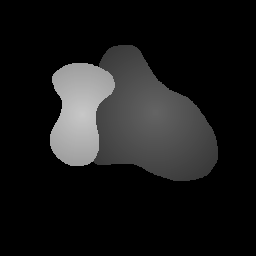
\includegraphics[height=.2\textheight]{background/background-segmentation-thresholding-binaryexample-a.png}}%
	%
	\hspace{4mm}%
	%
	\subfigure[The thresholded image]
	{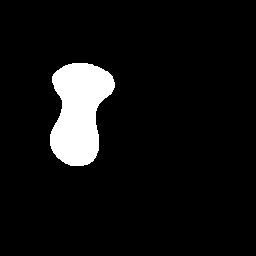
\includegraphics[height=.2\textheight]{background/background-segmentation-thresholding-binaryexample-b.png}}%
	%
	\hspace{4mm}%
	%
	\subfigure[The image histogram and threshold (at grey value $125$)]
	{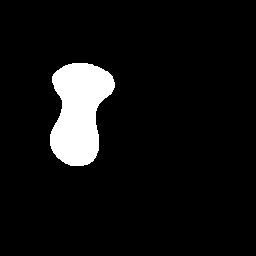
\includegraphics[height=.2\textheight]{background/background-segmentation-thresholding-binaryexample-c.png}}%
\caption{Segmenting the brighter of two adjacent objects in an 8-bit greyscale image using binary thresholding (the objects are easily separated in this case because the distribution of grey values in the image is bimodal)}
\label{fig:background-segmentation-thresholding-binaryexample}
\end{stusubfig}
%---

%---
\begin{stusubfig}{p}
	\subfigure[Segmenting Figure~\ref{fig:background-segmentation-thresholding-binaryexample}(a) with a threshold of $175$ leads to undersegmentation]
	{
\includegraphics[height=.2\textheight]{background/background-segmentation-thresholding-inaccurate-a.png}}%
	%
	\hspace{4mm}%
	%
	\subfigure[Conversely, segmenting it with a threshold of $75$ leads to oversegmentation]
	{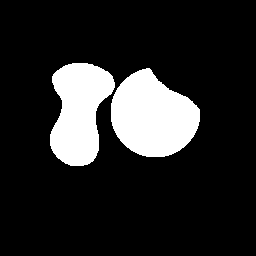
\includegraphics[height=.2\textheight]{background/background-segmentation-thresholding-inaccurate-b.png}}%
\caption{Misplaced thresholds lead to inaccurate segmentations}
\label{fig:background-segmentation-thresholding-inaccurate}
\end{stusubfig}
%---

\afterpage{\clearpage}

The difficulty encountered in practice is how to determine the optimum threshold location(s). A misplaced threshold will cause an inaccurate segmentation, so choosing the location appropriately is essential. In our example above, choosing a threshold that was too high would mean that the foreground of the image would be \emph{undersegmented} (i.e. pixels which should be classified as being part of the foreground are incorrectly classified as background) and the background would be \emph{oversegmented} (the converse) -- see Figure~\ref{fig:background-segmentation-thresholding-inaccurate}(a). Choosing too low a threshold would cause the opposite problem -- see Figure~\ref{fig:background-segmentation-thresholding-inaccurate}(b).

Owing to difficulties like this, applications are often designed so that thresholds can be chosen interactively by the user, but a great deal of work has also been done on automatically determining good threshold locations. As surveyed by Sezgin and Sankur in \cite{sezgin04}, there are six types of approach to the problem in current use:

\begin{enumerate}

\item \emph{Histogram shape-based methods.} These use shape properties of the histogram to find a good threshold. For instance, Rosenfeld's histogram concavity method, cited in \cite{lee.c92}, works by examining the difference between a histogram and its convex hull. A grey level at which the the height difference between the histogram and its convex hull is greatest (i.e. a point of deepest concavity) is picked as the threshold value.

\item \emph{Clustering-based methods.} These try and group the grey level data into a given number of clusters (two in the case of binary thresholding). One example is the method of Ridler and Calvard \cite{ridler78}. Their idea was to take a grey-level image and produce an initial binary classification which makes the assumption that the object of interest is somewhere in the middle of the image and the corners of the image contain only background. The means of the pixels currently classified as background and object are calculated and the average of the two means is taken. The new value is then used to threshold the image and produce a new binary classification into background and object classes: it is assumed that this will be more accurate than the initial guess. Finally, the process is iterated until there is little or no change in the binary classification, and the last threshold in the iteration is chosen for use.

\item \emph{Entropy-based methods.} These are based on information theory and pick thresholds by (for example) trying to maximise the information content in the thresholded image. As described by Wong and Sahoo in \cite{wong89}, the simplest possible such method looks at two probabilities, $F(T)$ and $F^*(T) = 1 - F(T)$, each parameterised in terms of a threshold, $T$. The first, $F(T)$, gives us the probability of a given pixel having a grey value less than or equal to the threshold, and the second, $F^*(T)$, gives us the probability of the value being greater than it. The information content in the thresholded image is given by
%
\[
H(T) = -F(T) \log_2 F(T) - F^*(T) \log_2 F^*(T)
\]
%
and attains a maximum when $F(T) = 0.5$. This is equivalent to saying that in the absence of any other knowledge, the maximum entropy principle tells us that the information contained in the thresholded image is maximised by picking a threshold which classifies half the pixels as background and half as foreground. This makes intuitive sense, but is too simplistic an approach for the majority of applications. Better alternatives have been developed (see \cite{sezgin04}), but are beyond the scope of this dissertation.

\item \emph{Object attribute-based methods.} These pick thresholds based on a comparison between the original grey-level image and the binarized (i.e.~segmented into two classes) version of it. For example, the method of Hertz and Schafer \cite{hertz88} picks the threshold that yields a binarized image whose edge field maximally corresponds to that of the original image. The edge fields in this case are obtained via the well-known Sobel operator \cite{gonzalez02}.

\item \emph{Spatial methods.} An example of a spatial thresholding method is Wu et al.'s approach in \cite{wu82}. This first constructs a quadtree from the image by splitting image regions until they have a low standard deviation (where they define `low' in terms of the standard deviation of the image as a whole). This divides the image into square blocks of various different sizes. The observation is that the smaller blocks tend to be near the boundaries between foreground and background in the image -- the quadtree can thus be used as a way of estimating where these boundaries are. Having classified the pixels in the image in this way, it is possible to construct a histogram of the grey values of non-boundary pixels in the image, which it is hoped will be more bimodal than the histogram of the grey values in the image as a whole. A threshold can then be placed at the deepest point in the value between the two modes. Alternatively, a histogram of the boundary pixels can be constructed, which it is hoped will be unimodal, and a threshold can be placed at the mean of this histogram instead.

\item \emph{Local / adaptive methods.} These vary the threshold for each pixel location in the image. Two examples of this are the methods of Bernsen \cite{bernsen86} and Niblack \cite{niblack86}. As described by Trier and Jain in \cite{trier95}, Bernsen's method takes the highest and lowest grey values, $g_{\mbox{max}}$ and $g_{\mbox{min}}$, in a suitably-sized window around each pixel, and uses them to calculate a contrast measure $C = g_{\mbox{max}} - g_{\mbox{min}}$. If $C$ is less than some user-specified value, the local neighbourhood around the pixel is taken to be uniform, and an appropriate choice is made about whether the pixel should be classified as background or foreground (in \cite{trier95}, pixels were always classified as background in this case). Otherwise, a threshold value $T = (g_{\mbox{max}} + g_{\mbox{min}}) / 2$ is calculated, and the pixel is classified as foreground if its value is greater than $T$, and background if not. Niblack's method, by contrast, bases its decision on the mean and standard deviation of the grey values in the local neighbourhood around a pixel. In particular, if $m$ is the local mean and $s$ the local standard deviation, Niblack's method calculates a local threshold $T = m + ks$, where $k$ is a (negative) user-specified parameter. Again, a pixel is classified as foreground iff its grey value is greater than $T$.

\end{enumerate}

\noindent In spite of the large amount of work done on thresholding, however, it has some significant downsides when used on its own to process medical images:

\begin{itemize}

\item It divides the image into two or more groups of pixels, based on their grey values, but there is no guarantee (or even an expectation) that any of these groups will be contiguous in the image. For instance, trying to segment a kidney from a CT scan by bounding it between two grey value thresholds might also result in inadvertently segmenting blood vessels across the image as well (their grey levels are quite similar to those of the kidneys). Not only are these blood vessels not part of the kidney, they are actually physically separated from it in the image! (It is also worth noting that trying to segment a kidney will generally result in segmenting both of them at once, since their grey level ranges are the same. This sort of problem can be overcome by specifying the side of the body in which we're interested.)

\item It is by no means the case that acceptable threshold locations always exist. If the grey value ranges of different objects of interest significantly overlap, it may be impossible to separate them using thresholding alone.

\end{itemize}

\noindent These limitations can in some cases be overcome by combining thresholding with other techniques. For instance, the results of thresholding often have gaps in them, which can sometimes be filled in by carefully applying various morphological operators (e.g. morphological opening and closing). Luc Soler's team \cite{soler01} made use of thresholding (as one technique among many) and achieved excellent automatic segmentation results for the liver. However, they did not use thresholding on its own. For instance, they segmented bones by thresholding for bright areas and then keeping only those which were near to the fat tissue (which had already been segmented). Simple thresholding alone would have been insufficient for the task, since structures such as the aorta also appeared bright on the contrast-enhanced images.

\subsection{Region Growing}

Region growing methods for segmentation essentially work as follows. First, an initial seed point is chosen for a feature of interest. Then, the region is `grown' by iteratively considering all points which are adjacent to the region and adding any which satisfy certain criteria (see Figure~\ref{fig:background-segmentation-regiongrowing-process}). For example, we could choose to add adjacent pixels whose grey value differs from that of their neighbour in the region by less than a certain amount. Alternatively, we could try and add adjacent pixels which preserve the homogeneity of the entire region (for some suitable definition of homogeneity) -- e.g.~Chen et al.\ \cite{chen09} define a criterion that leads an adjacent pixel to be added to the region provided that the absolute difference between its grey value and the mean grey value of the region is less than the standard deviation of the region's grey value distribution.

%---
\begin{stusubfig}{p}
	\subfigure[Initial state]
	{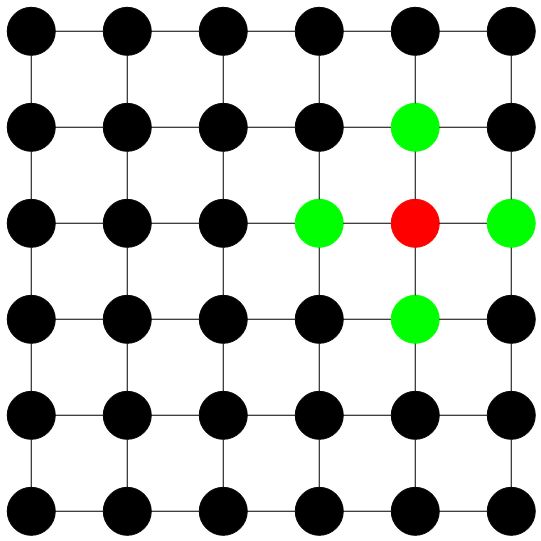
\includegraphics[height=5cm]{background/background-segmentation-regiongrowing-process-a.png}}%
	%
	\hspace{12mm}%
	%
	\subfigure[After one iteration]
	{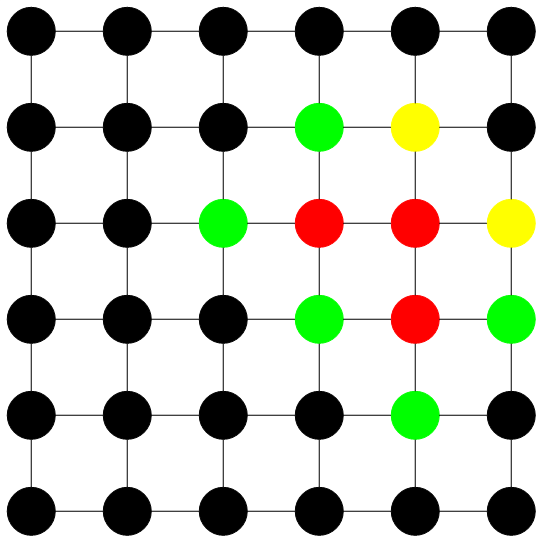
\includegraphics[height=5cm]{background/background-segmentation-regiongrowing-process-b.png}}%
	%
	\\ \vspace{12mm}
	%
	\subfigure[After two iterations]
	{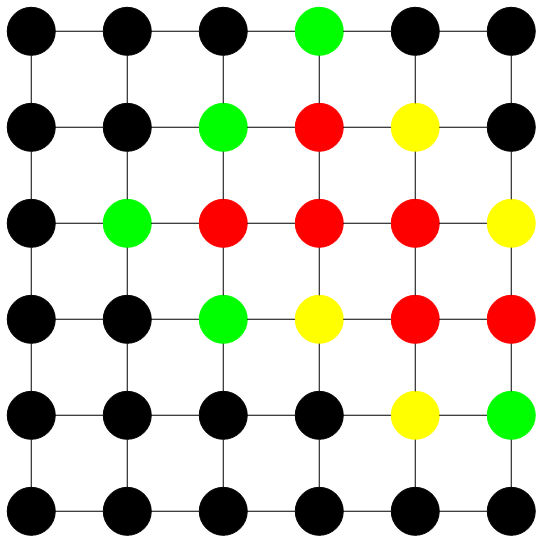
\includegraphics[height=5cm]{background/background-segmentation-regiongrowing-process-c.png}}%
	%
	\hspace{12mm}%
	%
	\subfigure[Final state]
	{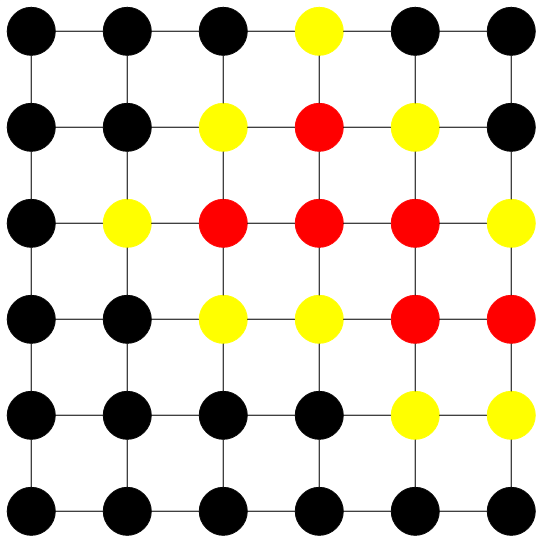
\includegraphics[height=5cm]{background/background-segmentation-regiongrowing-process-d.png}}%
\caption{An example region growing process -- black pixels are those not yet considered, red pixels are those currently in the region, green pixels are those under consideration, and yellow pixels are those that already failed the similarity criterion. The algorithm terminates when there are no further pixels to consider. The final segmented object is shown in red in (d).}
\label{fig:background-segmentation-regiongrowing-process}
\end{stusubfig}
%---

%---
\begin{stulisting}[p]
\caption{A Generic Region Growing Algorithm}
\label{code:background-segmentation-regiongrowing-generic}
\begin{lstlisting}[style=Default]
function grow_region
: (seed : PixelCoords; criterion : PixelCoords $\to$ bool) $\to$ Set<PixelCoords>

	var queue : Queue<PixelCoords>;
	var result, visited : Set<PixelCoords>;

	// Add the seed point to the queue and mark it as visited.
	queue.push(seed);
	visited.insert(seed);

	while not queue.empty()
		p := queue.pop();
		result.insert(p);

		// Add neighbours satisfying the similarity criterion to the queue.
		for each neighbour $\in$ neighbours(p)
			if not visited.contains(neighbour) then
				if criterion(neighbour) = true then queue.push(neighbour);
				visited.insert(neighbour);
			
	return result;
\end{lstlisting}
\end{stulisting}
%---

More involved criteria are also possible. One popular approach is that of \emph{adaptive} region growing (e.g.~see \cite{lin06,pohle01}), whereby the criterion varies to take account of the area around the pixel under consideration. In \cite{lin06}, for example, the approach taken is as follows. After locating an initial seed point $(s_x, s_y)$, a $7 \times 7$ mesh is placed over it and the maximum and minimum pixel intensities within the mesh, $M(s_x, s_y)$ and $m(s_x, s_y)$ are determined. From these, a contrast range $t_0 = M(s_x, s_y) - m(s_x, s_y)$ is calculated and recorded. Next, for each pixel $(x,y)$ under consideration for addition to the region, values $M(x,y)$ and $m(x,y)$ are similarly calculated, and a local value $\theta_{\rm local} = (M(x,y) + m(x,y)) / 2$ is determined. The region growing criterion is then formulated as $|f(x,y) - \theta_{\rm local}| \le t_0$, i.e. we add an adjacent pixel $(x,y)$ to the region if the absolute difference between its grey value $f(x,y)$ and the midpoint of the contrast range of the $7 \times 7$ mesh surrounding it is less than the contrast range of the $7 \times 7$ mesh centred on the initial seed point. The region growing is specified to stop when this absolute difference is greater than a certain threshold, implying that the area surrounding a given pixel is not homogeneous.

A generic region growing algorithm can be implemented straightforwardly using a queue (see Listing~\ref{code:background-segmentation-regiongrowing-generic}). Starting from a queue containing only the initial seed point, we repeatedly pop the pixel at the front of the queue, consider its non-region neighbours for addition to the region, and push any which satisfy the requisite criteria onto the end of the queue. The process terminates when the queue empties.

The key policy issues to consider when implementing region growing are how to choose the seed point, how to formulate the criteria specifying which points to add to the region, and how to decide when the process should terminate. For automated segmentation methods, how to choose the seed point is of fundamental importance; semi-automated algorithms can focus exclusively on the latter two problems, relying instead on the user to interactively specify an initial seed.

The advantages of region growing methods are that the resultant region is guaranteed to be connected in the image (unlike with thresholding) and that they are, on the whole, fairly easy to implement. However, from the point of view of automatic segmentation, they present difficulties, because choosing an initial seed point is in general a non-trivial problem. The usual approach taken for automatic seed point selection is to rely on statistical data about where the features of interest (e.g. organs) usually lie in the body. For instance, the approach in \cite{lin06} is to search for suitable seed points in two elliptical regions on each side of the body, one for each kidney. This worked quite well in context, but is not robust in the general case, relying strongly on the kidneys being in the expected places -- for example, it is unsuitable for MRI images, in which the patient's body may be oriented arbitrarily. It would also fail if used for images of auto-transplant patients.

Whilst region growing algorithms are guaranteed to produce a connected result, the region may still have holes in the middle of it. Whilst this may be desirable if we really are trying to segment a torus-shaped feature, on the whole it is necessary to post-process the region growing results to remove these holes, e.g.~using morphological closing techniques.

\subsection{Morphological Techniques}

Mathematical morphology is a large and rather general field based on lattice theory \cite{goutsias00}. It contains many useful image processing techniques, the majority of which are not relevant for the purposes of this survey, but in segmentation terms its key technique is the watershed transform, originally developed by Serge Beucher \cite{beucher90}.

The watershed, which will be described in substantially more detail in Chapter~\ref{chap:segmentation}, is essentially a technique for dividing landscapes into their catchment basins (where a catchment basin is an area of the landscape from which water would run down to a given local minimum) -- see Figure~\ref{fig:background-segmentation-watershed-concept}. In imaging terms, this can be utilised for segmentation purposes by treating an image as a discrete landscape and pre-processing it so as to try to establish a correspondence between catchment basins in the landscape and features of interest in the image. If such a correspondence can be successfully established, finding the catchment basins then equates to finding the desired image features.

%---
\stufigex{width=9cm, height=9cm}{segmentation/segmentation-watershed-concept.png}{The watershed transform constructs watersheds (the red partitions) that divide a landscape into its catchment basins}{fig:background-segmentation-watershed-concept}{p}
%---

Many image algorithms have been developed to actually perform the watershed transform; in general, these can be classified as either flooding algorithms (e.g.~\cite{bieniek00,rambabu07}) or rainfalling algorithms (e.g.~\cite{meijster98,osma-ruiz06,stoev00}). The former essentially flood out from the local minima in the landscape and (implicitly or otherwise) add watershed boundaries where the different catchment basins meet; the latter determine paths of steepest descent from points in the landscape and assign them to catchment basins based on the local minima to which their paths lead down.

In practice, however, it is rarely possible to establish a perfect correspondence between the catchment basins in the landscape and the desired features in the image, as to do so consistently would require prior knowledge of where the desired features actually are in the image, which would defeat the point of segmenting the image in the first place. One of the most common problems encountered with the watershed transform is that of oversegmentation: the landscape fed into the watershed has an excess number of catchment basins, most of which do not correspond to anything of interest in the actual image. This is particularly true of landscapes representing noisy images -- small changes in grey values can create shallow catchment basins, or dimples, in the landscape, greatly affecting the resulting segmentation.

There are two main approaches in the literature for dealing with this problem, namely marker imposition (leading to an approach known rather aptly as `watershed-from-markers') and hierarchical segmentation. Marker imposition essentially works by specifying markers on particular features of interest a priori, and flooding out only from those. This partitions an image into a number of regions equal to the number of specified markers and thereby solves the oversegmentation problem. Unfortunately, it can be extremely difficult to determine the required markers automatically -- rather than solving the underlying problem, we have merely changed it into one of marker determination. This may or may not prove problematic, depending on the data available and the specifics of the application. In some cases, it may be possible to use other data to determine marker placement automatically -- for example, Grau et al.\ \cite{grau04} successfully used a statistical atlas for this. In other cases, it may simply be acceptable to place the markers manually \cite{xue05}, or to initially place them manually and then propagate them from one image in a sequence to the next \cite{flores09}.

In situations where neither is the case, however, the alternative approach of hierarchical segmentation can be used. As one might expect, the general idea here is to take the oversegmented result of running the watershed transform on an image, and perform several iterations of region merging to produce a hierarchy of gradually coarser partitions of the original image. As will be illustrated in far more detail in Chapter~\ref{chap:segmentation}, this is exactly the sort of approach taken by the waterfall transform \cite{beucher90,marcotegui05}: what is unique about the waterfall, however, is that each of its iterations in which it merges regions together is itself a watershed transform.

As will be discussed in Chapter~\ref{chap:methodology}, the hierarchical approach to watershed segmentation is interesting for a couple of reasons: on the one hand, it produces, without requiring a great deal of manual fine-tuning, segmentations which, whilst not perfect, are often quite reasonable to a first approximation; on the other hand, the hierarchy of partitions of the image it produces can be turned into a tree structure (see \S\ref{sec:background-partitionhierarchies}) which is amenable to further editing, allowing any flaws in the initial segmentation to be corrected in an intuitive manner. These two qualities make this approach eminently suitable in situations where automated solutions are desirable but interactive control remains important.

\subsection{Deformable Models}

As their name suggests, deformable models methods work by taking an initial model of the features under consideration and deforming it to fit the actual data available. The initialisation of the model is generally based on \emph{a priori} anatomical knowledge. The model itself can be represented in a variety of ways, and these ways correspond to a number of different approaches to the problem. For example, the snakes method, which we will see shortly, represents the model as a parametrically-defined spline, and is hence referred to as an example of a parametric deformable model (it is sometimes also referred to as an explicit deformable model). In contrast, level sets represent the model \emph{implicitly} and are an example of implicit deformable models. Implicit deformable models were developed later than their parametric counterparts, but both types see a lot of use.

\subsubsection{Parametric Deformable Models}

\paragraph{Snakes}

As originally defined by Kass, Witkin and Terzopoulos in \cite{kass88}, `A snake is an energy-minimizing spline guided by external constraint forces and influenced by image forces that pull it toward features such as lines and edges.' Essentially, the idea works as follows. We represent the position of the snake, in terms of a spline parameter $s$, as $\mathbf{v}(s) = (x(s),y(s))$, and define an \emph{energy functional}, $E_{snake}^*$, as
%
\[
E_{snake}^* = \int_0^1 E_{int}(\mathbf{v}(s)) + E_{image}(\mathbf{v}(s)) + E_{con}(\mathbf{v}(s)) \; ds.
\]
%
The three terms in the summation are \emph{internal} energy, which tries to limit the curvature of the snake, \emph{image} energy, which tries to attract the snake towards features in the image such as lines and edges, and \emph{constraint} energy, which allows the user to apply constraints to influence the result of the segmentation. The snake algorithm as a whole attempts to find a spline minimising $E_{snake}^*$.

The original snakes paper describes a continuous model, but more recent research \cite{lobregt95,miller90b,miller90a} has seen the development of discrete models as well. The model described by Lobregt and Viergever in \cite{lobregt95}, called a \emph{discrete dynamic contour model}, is particularly interesting, and worth describing in more detail. Rather than relying on ideas of energy-minimization, Lobregt and Viergever model snakes using a force-based physical simulation. In their approach, a snake is a set of vertices connected by edges. At each time-step, various forces are applied to each vertex, which gradually \emph{deform} the snake towards the desired result. The results of this approach will depend to an extent on the lengths of the edges joining the vertices: if an edge is too long, important image features may pass through the gaps between vertices; if it is too short, the snake may become overly fixated on small details, not to mention the speed of the process being adversely affected. For this reason, after each deformation step, the snake is \emph{resampled} (by adding or removing vertices where necessary) to keep the edge lengths within certain limits.

The forces applied to each vertex closely mimic the energy terms in the original snakes paper. The force $\mathbf{f_i}$ applied to vertex $i$ is defined as the weighted sum
%
\[
\mathbf{f_i} = w_{ex}\mathbf{f_{ex,r_i}} + w_{in}\mathbf{f_{in,i}} + \underbrace{w_{damp}}_{< \; 0}\mathbf{v_i},
\]
%
where $\mathbf{f_{ex,r_i}}$ is an \emph{external} force term corresponding to the image and constraint terms from the original formulation, $\mathbf{f_{in,i}}$ is an \emph{internal} force term corresponding to the original internal term, and the remaining term is a new addition used to apply damping to try and bring the simulation to rest. (The real numbers $w_{ex}$, $w_{in}$ and $w_{damp}$ specify the weights to be given to each of these three factors. The paper tended to set all three of these to $0.5$: apparently this was derived empirically.)

It is important to mention that the method relies on quite a close initialisation (i.e.~image features have quite a short capture range). In \cite{ree05}, this problem is circumvented by peforming a watershed-from-markers segmentation and using the result of that to initialise the snake. Another alternative, referred to there, is to try and add additional external forces to solve the problem: in particular, some success has been had with \emph{balloon forces} \cite{cohen91} and \emph{gradient vector flow} (GVF) \cite{xu98}. For example, Figure~\ref{fig:background-segmentation-snakes-gvfexample} shows a GVF snake successfully segmenting the left ventricle of a human heart.

%---
\stufigex{height=9cm}{background/background-segmentation-snakes-gvfexample.png}{The basic snakes method suffers from a poor capture range, but techniques such as gradient vector flow \cite{xu98} can mitigate this -- the figure (reproduced from the paper in question) shows a GVF snake deforming from an initial, circular contour to segment the left ventricle of a human heart }{fig:background-segmentation-snakes-gvfexample}{p}
%---

Problems of this kind with snakes methods have led to a great deal of interest in level sets as an alternative, although snakes also remain popular as a well-established and far simpler alternative. They also have the advantage that they can represent open structures as well as closed ones.

\paragraph{NURBS-Based}

Another type of parametric deformable model, this time based on non-uniform rational B-splines (NURBS), is described by Tsagaan et al.\ \cite{tsagaan02}, in which they use a 3D NURBS-based model of a kidney and deform it by minimizing an energy function. Their results seem good in some cases, but differ markedly from the manually segmented results they show in others.

\subsubsection{Implicit Deformable Models}

\paragraph{Level Sets}

Curves and surfaces in general can be specified either explicitly (such that they can be calculated directly from the definition) or implicitly (the opposite). For instance, an explicit (parametric) representation of a circle in terms of its radius $r$ and an angle $\theta$ might be:
%
\begin{eqnarray*}
x & = & r \cos \theta \\
y & = & r \sin \theta
\end{eqnarray*}
%
The corresponding implicit representation would be:
%
\[
x^2 + y^2 = r^2
\]
%
As we have seen, parametric deformable model approaches like snakes represent their model using the former approach. Level set approaches, by contrast, use the latter. As an introduction to the ideas behind level sets, consider the function $\psi(x,y) = x^2 + y^2$, which defines a scalar field over $\mathbb{R}^2$. For any value $k > 0$, the equation $\psi(x,y) = k$ defines a circle in the x-y plane: we will refer to each of these circles as an \emph{isosurface} of $\psi$, because each of them is the surface (curve) of all the points at which $\psi$ takes a particular value.\footnote{\emph{Iso} means `equal' in Greek, so here we are talking about the surface containing all the points with the same $\psi$ value.} The key idea is that if we now change $\psi$, for instance by redefining it as $\psi(x,y) = x^3 + y^3$, the isosurfaces change, in this case from circles to hypercircles. Thus by changing the function $\psi$, we can move the isosurfaces of $\psi$ around without ever having to represent them explicitly. Level set approaches make use of this by representing the deformable model as an isosurface of some function $\psi$, and then modifying $\psi$ to deform the model towards the boundary of the desired image feature.

%---
\stufigex{height=6cm}{background/background-segmentation-levelsets-circleexample.png}{A simple circular contour which gradually expands over time}{fig:background-segmentation-levelsets-circleexample}{p}
%---

%---
\stufigex{height=6cm}{background/background-segmentation-levelsets-ellipseexample.png}{An example of a contour which changes its shape over time}{fig:background-segmentation-levelsets-ellipseexample}{p}
%---

%---
\stufigex{height=6cm}{background/background-segmentation-levelsets-uniformgrid.png}{Approximating a function $\psi(\mathbf{x},t)$ with a discrete, uniformly-spaced grid (note that the time superscripts on the grid values are not shown)}{fig:background-segmentation-levelsets-uniformgrid}{p}
%---

To represent contour changes over time, level set approaches make $\psi$ a function of time as well, and define it over some domain $U \subset \mathbb{R}^N$, giving us $\psi(\mathbf{x}, t) : U \times \mathbb{R}^+ \rightarrow \mathbb{R}$. They then set this equal to some constant (generally $0$) to actually specify one of the isosurfaces of $\psi$ as the contour being deformed. As a simple example of this, consider a circle, centred at the origin, which gradually expands outwards as the time increases (see Figure~\ref{fig:background-segmentation-levelsets-circleexample}). Supposing its radius to be $t$ at time $t$, we could represent this as:
%
\[
\psi((x,y),t) = x^2 + y^2 - t^2 = 0
\]
%
A more complicated example might involve gradually changing the circle into an ellipse over time (see Figure~\ref{fig:background-segmentation-levelsets-ellipseexample}). This could be achieved by writing:
%
\[
\psi((x,y),t) = x^2 + (yt)^2 - t^2 = 0
\]
%
Thus far, we have examined the basic ideas underpinning level sets, but not seen how they can be applied to the practical problem of segmentation. A common approach of real-world level set methods is to take as input not an explicit function of the kind we have just seen, but an initial contour on the image. This will then be deformed (using numerical methods) over time to try and fit it to an image feature of interest. There are thus six essential questions to consider:

\begin{enumerate}

\item How do we represent the function $\psi$?

\item Given an initial contour by the user, how do we use it to construct the initial function $\psi(\mathbf{x}, t = 0)$?

\item How do we define a numerical method to deform the initial function over time?

\item How do we know when the algorithm has terminated?

\item How do we extract the contour of interest over time?

\item How do we try and make the algorithm segment the desired image feature?

\end{enumerate}

\noindent To answer these questions, we consider the level set approach of Malladi et al., described in \cite{malladi95}. There, as tends to be the case for level set approaches in general, the function $\psi$ is represented by storing a discrete grid of approximate values over the domain $U$. The grid is uniformly-spaced, with squares of side $h$ (see Figure~\ref{fig:background-segmentation-levelsets-uniformgrid}). Each grid node has (for each integer value of $n \ge 0$) an associated value $\psi_{ij}^n$, which approximates the value $\psi((ih,jh),n\dt)$, where $\dt$ is the time step of the numerical method that will be used to deform the initial contour over time.

The initial goal is to construct, from a contour specified by the user, the grid of values $\psi_{ij}^0$ approximating the function $\psi(\mathbf{x},0)$. In \cite{malladi95}, this is done by setting $\psi_{ij}^0$ to be the signed distance of the grid node $ij$ from the initial contour (points outside the contour are assigned positive values and those inside are assigned negative ones) -- see Figure~\ref{fig:background-segmentation-levelsets-initialfunction}.

%---
\stufigex{height=7cm}{background/background-segmentation-levelsets-initialfunction.png}{Generating the initial function from the zero contour specified by the user (in red)}{fig:background-segmentation-levelsets-initialfunction}{p}
%---

Having constructed the grid for the initial function, the next step is then to define an appropriate numerical method to deform it over time. To do this, we first need a partial differential equation for $\psi$. The appropriate PDE, as derived in \cite{malladi95}, is:
%
\[
\pd{\psi}{t} + F|\nabla \psi| = 0
\]
%
Here, $F$ is called the \emph{speed function}, and will be used to control how $\psi$ evolves in a manner that will be discussed below. This can be approximated numerically as
%
\[
\frac{\psi_{ij}^{n+1} - \psi_{ij}^n}{\dt} + (F)(\nabla_{ij} \psi_{ij}^n) = 0,
\]
%
where (as noted, and described in more detail, in the paper), $\nabla_{ij} \psi_{ij}^n$ is `some appropriate finite difference operator for the spatial derivative'. This equation can be iteratively solved using standard numerical techniques (e.g.~see \cite{morton05}) and used to deform the model over time. The algorithm terminates when the contour of interest no longer changes between iterations.

To extract the contour of interest after each iteration, Malladi et al. construct a piecewise linear approximation to it, the gist of which involves finding the squares where some of the corner values are positive and some are negative, and constructing line segments therein. This bears not a little resemblance to the marching squares algorithm, the 2D analogue of marching cubes \cite{lorensen87}.

The remaining issue is how to use this algorithm to actually segment features in an image. For this, we make use of the speed function $F$, which controls how the contour deforms. Malladi et al.\ go into great detail about how $F$ should be defined, but essentially the idea is to define it so as to have (a) an advection component -- basically a term providing a constant speed inwards or outwards, (b) an image component -- a term which tries to make the contour move quickly when it is not near potential feature boundaries and slowly when it is close to them, and possibly (c) a geometry component -- a term which aims to control the local curvature of the contour. For the two-component version, with only an advection and an image component, this corresponds to an equation of the form
%
\[
\pd{\psi}{t} + (F_A + \hat{F}_I)|\nabla \psi| = 0,
\]
%
where $F_A$ is the advection component and $\hat{F}_I$ is the image component. For the version with a geometry component as well, the equation becomes
%
\[
\pd{\psi}{t} + \hat{k}_I(F_A + F_G)|\nabla \psi| = 0,
\]
%
where $F_G$ is the geometry component and $\hat{k}_I$ fulfils the role of the image component in the previous equation. The detailed definitions of the various components can be found in \cite{malladi95}. It is worth noting that this term-based approach bears a lot of similarity to that used for snakes, and in general the motivations for the various terms are more or less the same in each case.

Level sets have a number of advantages over snakes. One advantage is that they handle topological changes in an extremely simple fashion. For instance, consider Figure~\ref{fig:background-segmentation-levelsets-topologychanges}(a), in which the isosurface $\psi = 4$ is divided into two separate components. This is seamlessly represented by a level set approach, since it merely has to maintain a grid of numbers and not one or more explicit curves. Furthermore, the number of components can evolve over time without any special handling being required: in Figure~\ref{fig:background-segmentation-levelsets-topologychanges}(b), a change to the value of a single grid point can merge the two separate components into one, changing the topology at a stroke without any fuss. A corresponding implementation with snakes would involve far more work.

%---
\begin{stusubfig}{p}
	\subfigure[An isosurface divided into two separate components]
	{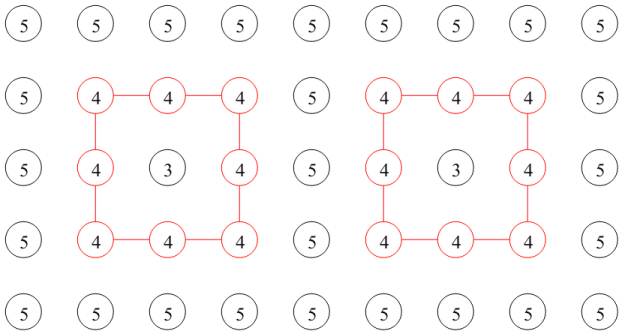
\includegraphics[height=6cm]{background/background-segmentation-levelsets-topologychanges-a.png}}%
	%
	\\ \vspace{4mm}%
	%
	\subfigure[Changing a single grid value merges the two components into one]
	{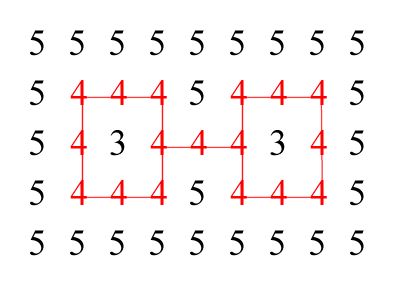
\includegraphics[height=6cm]{background/background-segmentation-levelsets-topologychanges-b.png}}%
\caption{Level set approaches seamlessly handle multiple boundaries and changes in topology}
\label{fig:background-segmentation-levelsets-topologychanges}
\end{stusubfig}
%---

Another advantage of level sets is that, unlike snakes, they translate straightforwardly into three dimensions -- all that is required is to replace a 2D grid with a 3D one. It is worth remarking, however, that the extra processing involved in the 3D case is substantial, making the basic scheme described above unsuitable if timely solutions are required. Special techniques have been developed to deal with this problem. One example is the narrow-band technique mentioned in \cite{malladi95}, which essentially restricts numerical calculations to a narrow regions around the isosurface in which we're particularly interested (i.e.~the one representing the deformable model). The insight is that solving the PDE over the whole domain is only necessary if we're interested in solving for the entire family of isosurfaces associated with $\psi$: often, we're only interested in a single isosurface, so the extra computations aren't necessary. More details of this sort of technique are available in \cite{malladi95} and \cite{itk}.

\subsubsection{Other Deformable Models}

Although parametric and implicit models are the most common types of deformable model in use, there are some techniques which do not fall into either category. Two techniques in particular are worth briefly mentioning. In \cite{jalba04}, Jalba et al.\ use a deformable model based on charged particles to achieve some interesting automatic segmentation results. There, the model is represented neither parametrically nor implicitly, but instead as a set of charged particles under the influence of an electrostatic field. Another interesting type of deformable model is the m-rep, described by Pizer et al.\ in \cite{pizer03}. This uses a medial representation of the model.

\subsection{Learning Techniques}

Learning segmentation techniques generally start with a training phase, in which a large number of scans are taken and used to construct some variety of model, which encodes information that can be used to segment subsequent scans. Two different types of learning technique will be discussed in the following subsections.

\subsubsection{Atlas-Based Techniques}

Atlas-based methods start by constructing an atlas, or reference segmentation, from a set of training data. For instance, in \cite{park03}, Park et al.\ constructed a probabilistic atlas by registering (aligning) the manually segmented volumes of 31 patients onto that of a carefully chosen reference patient (thus the data came from 32 patients in all). The atlas was represented as a 3D grid of vector values, where the components of each vector corresponded to the organs under consideration, and the values of the components indicated the fractional percentage of registered data sets in which the point was labelled as the given organ. As an example, if we were considering the liver and the two kidneys, the vector $(0.4, 0.6, 0)^T$ at a point could indicate that the point was inside the liver in 40\% of the data sets and inside the right kidney in 60\% of them.

After constructing such an atlas, new sets of data can be segmented by registering them onto it. In \cite{park03}, they use a \emph{maximum a posteriori} (MAP) approach after registration to find the segmentation result which best explains the observed data. The important point here is that the segmentation result is based on both the data for the individual patient and the information encoded in the atlas. The atlas provides the prior probabilities at each voxel, and these are refined in light of the actual patient data.

To use the notation in \cite{park03}, we denote the segmentation result field as $\mathbf{X}$, the field of observed data for the individual patient as $\mathbf{Y}$, and the probabilistic atlas as $\mathbf{A}$. Each of these represents a volume of $N$ voxels, indexed linearly (in some order) from $1$ to $N$. So for instance, a particular segmentation result could be given by $\mathbf{x} = (x_1, x_2, \ldots, x_N)$. Our aim is to find the best possible $\mathbf{x}$, defined as
%
\[
\mathbf{\hat{x}} = \argmax_{\mathbf{x}} \mathbf{P}(\mathbf{X} = \mathbf{x} | \mathbf{Y} = \mathbf{y}).
\]
%
In other words, we seek the segmentation result which best explains the observed patient data, $\mathbf{y}$. The probabilistic atlas is used in all of this as the prior for $\mathbf{X}$. Suppose there are $L$ different possible voxel labels, numbered from $1$ to $L$. Each voxel $a_i$ of the probabilistic atlas contains an $L$-vector, $(a_{i,1}, \ldots, a_{i,L})$, where $a_{i,\ell}$ gives the probability of a voxel's correct label being $\ell$. We use this to define the prior probabilities for $\mathbf{X}$, writing
%
\[
P(x_i = \ell) = a_{i,\ell}.
\]
%
In other words, the probability of the correct segmentation result for a given voxel being $\ell$ is given by the $\ell^{th}$ component of the probabilistic atlas at that location. With this link made, the result determined will depend on both the atlas and the observed data.

\subsubsection{Neural Network Techniques}

Neural networks (NNs) can be used to segment images in a number of ways. A simple NN technique can be found in \cite{tsai94}, where Tsai and Tanahashi use a feed-forward network to classify each pixel into one of three classes (liver, boundary or non-liver) according to the grey-level histogram of the 7x7 region centred on the pixel. (In practice, they use a histogram with 16 grey levels instead of 256, to avoid a proliferation of input nodes in the NN.) The schematic of how this works (borrowed from their paper) is shown in Figure~\ref{fig:background-segmentation-neuralnets-tsai}. The NN is initially trained by picking a suitable image from the middle of the volume and marking a significant number of training regions for each class. The well-known back-propagation algorithm for NNs \cite{aima} is used to update the weights on the network arcs accordingly.

%---
\stufigex{height=20cm}{background/background-segmentation-neuralnets-tsai.png}{Schematic diagram of the neural-network-based boundary detection method used in \cite{tsai94} (reproduced from the paper in question)}{fig:background-segmentation-neuralnets-tsai}{p}
%---

A more up-to-date (and more complicated) NN scheme can be found in \cite{lee03}. Here, Lee et al.\ use a multi-module, recurrent neural network to segment multiple abdominal organs (see Figure~\ref{fig:background-segmentation-neuralnets-lee}). There is a module associated with each label under consideration. Each node of a given module $k$ corresponds to a pixel in the image and encodes the probability that the pixel should be assigned label $k$. The weights of the network arcs are initially derived from (for example) a correlation matrix containing the likelihoods of various labels occurring next to each other. (For example, the liver might be quite likely to occur next to the right kidney, but definitely shouldn't occur next to the left kidney.) An iterative state evolution algorithm is used to determine the probabilities at each node in each of the modules of the NN. The initial probabilities are generated using something called the `Kohonen self-organizing algorithm' (see the paper for details) and the nodes are updated at each time step based on the current probability at a given node and the support it receives from its neighbours. (So, for instance, if a pixel was currently classified as part of the left kidney, but all its neighbours were liver, it would be very likely to change to liver over time.) The results of this method (after combining it with fuzzy spatial rules for organ identification) are quite good -- see Figure~\ref{fig:background-segmentation-neuralnets-leeresults}.

%---
\stufigex{height=8cm}{background/background-segmentation-neuralnets-lee.png}{The architecture of the contextual neural network used in \cite{lee03} (reproduced from the paper in question)}{fig:background-segmentation-neuralnets-lee}{p}
%---

%---
\stufigex{height=8cm}{background/background-segmentation-neuralnets-leeresults.png}{Results of the neural network method described in \cite{lee03} (reproduced from the paper in question), showing the identified spine, left kidney, spleen and liver}{fig:background-segmentation-neuralnets-leeresults}{p}
%---

%\subsubsection{Statistical Methods}

%TODO: \cite{touhami05}

\subsection{Clustering}

Clustering is the general problem of how to collect objects into groups in such a way that the members of each group are (with relation to application-specific criteria) similar to each other, but dissimilar to those in other groups. This can evidently be applied to image segmentation, with the goal of clustering the image into groups of similar pixels.

\subsubsection{K-Means}

A generalised description of the K-means approach to clustering is that it aims to divide a set of $n$ objects $\{o_1,\ldots,o_n\}$ into $k \le n$ groups $G = \{G_1,\ldots,G_k\}$ in such a way as to minimise the sum of squares of some measure of similarity $m$ between each object and the `mean' of the objects of its group. (At this stage of the description, what is meant by the mean in this instance is left deliberately under-specified.) More formally, if $\mu_j$ is the mean of the objects in group $G_j$, K-means aims to find a set of groups $G$ minimising:
%
\[
\sum_{j=1}^k \sum_{o \in G_j} m(o, \mu_j)^2
\]
%
The method generally used to try and find $G$ is an heuristic known as Lloyd's algorithm \cite{lloyd82} (which, it must be remarked, may be difficult to discern from the original paper). This works as follows:

\begin{enumerate}

\item An initial set of $k$ means are chosen, either manually, randomly or otherwise.

\item Each object (in the case of imaging, each pixel) is assigned to the group to whose mean it is closest, i.e.~object $o$ is placed in the group with index:
%
\[
\argmin_{i=1}^k m(o, \mu_i)
\]

\item The means for all groups that have changed since the last iteration are recalculated.

\item Steps 2 and 3 are repeated until no groups change between one iteration and the next.

\end{enumerate}

\noindent Lloyd's algorithm is not guaranteed to find the global optimum for $G$, but it has been shown by Arthur and Vassilvitskii \cite{arthur07} that a careful choice of the initial means can make the algorithm $O(\log k)$-competitive with the optimal clustering.

The key issues when using Lloyd's algorithm to segment images are how to define both the similarity measure and the mean of a set of objects. In some domains, the similarity measure can simply be defined as the distance between objects, and the mean as the average of the objects' positions, but for images this may not produce good results. Instead, similarity measures can be defined which are based not only on the positions of the pixels, but also on their values (for example, see \cite{?}). In such cases, the way in which the mean of a set of objects is defined will vary accordingly.

It should be noted that each cluster produced by this simple k-means approach is highly unlikely to be contiguous in the image (see Figure~\ref{fig:background-segmentation-kmeans-noncontiguity}). Some attempts have been made to address this in the literature (e.g.~see \cite{luo03,ilea06}).

\subsubsection{Fuzzy C-Means}

Fuzzy C-means is essentially a fuzzy relative of the K-means approach just described. It was originally presented by Dunn in 1974 \cite{dunn74}. The key idea is that instead of objects being divided crisply into groups (i.e.~each object belonging completely to exactly one group), objects have a degree of membership for each group. Using the same notation as before, and letting $u_{ij}$ be a real number between $0$ and $1$ indicating the degree to which object $o_i$ is a member of group $G_j$, and $1 \le p < \infty$ be a real parameter (e.g.~$p = 2$), we seek to find a set of groups $G$ minimising:
%
\[
\sum_{j=1}^k \sum_{o_i \in G_j} u_{ij}^p \cdot m(o,\mu_j)^2
\]
%
The standard algorithm for fuzzy C-means is once again an iterative, heuristic method:

\begin{enumerate}

\item Initialise the $u_{ij}$ values for the first iteration (written as ${}^{(0)}u_{ij}$). Any of the initialisation approaches which work for K-means will work equally well for this (i.e.~it suffices to pick an initial set of means and assign objects completely to their nearest groups by setting the $u_{ij}$ value to $1$ for their group and $0$ for all other groups).

\item At iteration $s$, calculate the updated means of the groups using the equation:
%
\[
\mu_j^{(s)} = \frac{\displaystyle \sum_{o_i \in G_j} {}^{(s-1)}u_{ij}^p \cdot o_i}{\displaystyle \sum_{o_i \in G_j} {}^{(s-1)}u_{ij}^p}
\]

\item Calculate the updated values ${}^{(s+1)}u_{ij}$ using the equation:
%
\[
{}^{(s+1)}u_{ij} = \frac{1}{\displaystyle \sum_{j=1}^k \left( \frac{m(o_i, \mu_j)}{m(o_i, \mu_k)} \right)^{\frac{2}{p-1}}}
\]

\item Iterate Steps 2 and 3 until
%
\[
\max_{ij} |{}^{(s+1)}u_{ij} - {}^{(s)}u_{ij}| < \epsilon,
\]
%
where $\epsilon$ is a real number between $0$ and $1$.

\end{enumerate}

\noindent Once again, as with Lloyd's algorithm for K-means, this is not guaranteed to produce the global optimum.

\subsection{Graph Partitioning}
\label{subsec:graphpartitioning}

Graph partitioning segmentation algorithms work by representing an object to be segmented as a weighted, undirected graph. In the case of images, the nodes of this graph would be the pixels of the image, and each of its edges would connect a pair of adjacent pixels and be weighted according to some measure of the dissimilarity between those pixels (one possible definition, based on both the pixel values and their spatial location in the image, appears in \cite{shi00}). The idea is then to find a good way to partition the nodes of the graph into pieces. For instance, if $G = (V,E,w)$ is a graph with vertex set $V$, edge set $E$ and weight function $w$, the \emph{minimum cut} approach seeks to partition $V$ into two disjoint sets $A$ and $B$ such as to minimise:
%
\[
\mbox{cut}(A,B) = \sum_{u \in A, v \in B} w(u,v)
\]
%
As mentioned by (among others) Shi and Malik in \cite{shi00}, however, the minimum cut approach tends to partition the graph so as to cut away small groups of poorly connected nodes, with undesirable results. Instead, they define, and then try to minimise, a measure of the lack of quality of a binary partition called the \emph{normalized cut}, namely
%
\[
\mbox{Ncut}(A,B) = \frac{\mbox{cut}(A,B)}{\mbox{assoc}(A,V)} + \frac{\mbox{cut}(A,B)}{\mbox{assoc}(B,V)},
\]
%
where they define $\mbox{assoc}(X,V) = \sum_{u \in X, t \in V} w(u,t)$ for both $X = A$ and $X = B$. This solves the aforementioned problem with the minimum cut approach, because if (for example) $A$ is a small group of poorly connected nodes, we would expect $\mbox{cut}(A,B)$ to be almost the same as $\mbox{assoc}(A,V)$, leading to a large value for $\mbox{Ncut}(A,B)$.

Finding a good partition given the definition of a normalized cut involves solving an eigenvalue problem, the details of which are described in \cite{shi00}. Having solved the eigensystem, we take the second smallest eigenvector (for reasons discussed in the paper) and use it to try and compute a good partition. The eigenvector will have one real-valued component for each pixel in the image -- the idea is to find a splitting point which minimises the value of the normalized cut. Assuming the values are relatively well separated into two distinct clusters, this can be done by checking the cut value for a number of evenly-spaced, real-valued potential cut points, and picking the one with the lowest value. Pixels with values above the cut then form one group, and those with values below the other. If the values are not well separated, however, the cut values may well be similar for several different cut points. For that reason, \cite{shi00} defines a stability criterion which essentially measures the reliability of the cut.

The binary partitioning process thus far described then becomes part of a recursive partitioning scheme. Starting with the whole image, as good a binary partition as possible of the current image region is computed, along with the stability of the cut. If the stability is too low, the image region is not partitioned. Otherwise, the value of the cut itself is considered. If it is too high (i.e.~greater than some user-specified threshold), the recursion terminates. Otherwise, the binary partitioning process is repeated on the two sub-regions just computed. Via this recursive process, the image as a whole is partitioned into a number of groups dependent on the maximum allowed cut value and the stability criterion.

\subsection{Hybrid Techniques}

It is sometimes possible to achieve better results by combining a number of different segmentation methods than it is by using a single method on its own. A striking example of how successful this sort of technique can be seen in the work of Luc Soler et al.\ \cite{soler01}, in which they describe an extensively hybrid technique for automatic segmentation of the liver from spiral CT scans. Their segmentation method first uses thresholding, morphological operators and distance maps to identify the skin, bones, lungs, kidneys and spleen. They next use a clever deformable model approach to embed a reference model of the liver into the image and automatically deform it to the liver contours. Later stages use Gaussian fitting on the image histogram to separate normal liver tissue from blood vessels and lesions (tumours), a result which is further refined by their own analytical methods. The final stage of their method makes use of higher-level medical knowledge to label the hepatic portal vein and segment the liver automatically according to an anatomically-based definition by Couinaud \cite{couinaud57}. The results of this technique are excellent -- see Figure~\ref{fig:background-segmentation-hybrid-soler}.

%---
\stufigex{height=8cm}{background/background-segmentation-hybrid-soler.png}{An automatic 3D reconstruction of patients from medical images, as performed by the IRCAD surgical planning tools developed using the work of Luc Soler et al.\ (the figure is reproduced from \cite{soler-imvie})}{fig:background-segmentation-hybrid-soler}{t}
%---

Other hybrid methods can be found in e.g.~\cite{ng06} and \cite{itk}. In \cite{ng06}, Ng et al.\ precede a watershed segmentation of MRI images of the head with a K-means clustering step -- this has the effect of hugely reducing the oversegmentation that the watershed would otherwise produce. It is a method that works particularly well for head segmentation, where the number of clusters is well-known a priori (in this case, the authors note that the types of tissue present tend to be `bone, soft tissue, fat and background'). There are several hybrid segmentation methods in \cite{itk}: in one, the authors combine fuzzy connectedness, Voronoi diagram classification and deformable models; in another, they combine Gibbs priors and deformable models. The details of these techniques are beyond the scope of this dissertation, but an implementation of the methods can be found in the freely-available \emph{Insight Toolkit}.

\clearpage

%---
\section{Partition Hierarchies}
\label{sec:background-partitionhierarchies}

%TODO: (i) Brief description of what a partition tree is; (ii) Explain, with suitable references, the various situations in which they are used; (iii) Narrow it down to images and survey the various techniques, noting the key differences between the representations (e.g.~whether or not adjacency information is maintained, etc.); (iv) Explain (at a high level) how partition forests fit into the picture

\subsection{Overview}

Partition hierarchies comprise two related data structures -- partition trees and partition forests. A \emph{partition tree} is a tree-based data structure containing nodes that represent portions of an entity, and satisfying the condition that the sub-entities represented by the children of any node in the tree partition the sub-entity represented by that node -- that is, the child sub-entities together form the parent sub-entity, and none of the child sub-entities mutually overlap. (I will henceforth, for reasons of brevity, refer to nodes partitioning each other, rather than referring to the sub-entities they represent.) An example of a partition tree can be seen in Figure~\ref{fig:background-partitionhierarchies-treeexample}. Partition forests will be discussed below (and in Chapter~\ref{chap:ipfs}).

%---
\stufigex{height=8cm}{todo.png}{TODO}{fig:background-partitionhierarchies-treeexample}{p}
%---

Partition trees can be either incomplete or complete. An incomplete partition tree is one with an incomplete lowest layer, and a complete one is the opposite. Complete partition trees have the property that the nodes in any given layer form a partition of the entity as a whole. For either type of tree, this is also true of the set of leaf nodes (those nodes without children). It should be noted that every incomplete partition tree has an equivalent complete partition tree. This can be constructed by adding a chain of nodes downwards from every leaf which is not in the lowest layer -- see Figure~\ref{fig:background-partitionhierarchies-completeness}.

%---
\begin{stusubfig}{p}
	\subfigure[An incomplete partition tree]
	{
\includegraphics[height=8cm]{todo.png}}%
	%
	\hspace{4mm}%
	%
	\subfigure[The same tree after making it complete]
	{
\includegraphics[height=8cm]{todo.png}}%
\caption{Any incomplete partition tree can be converted into a complete one}
\label{fig:background-partitionhierarchies-completeness}
\end{stusubfig}
%---

There are essentially two ways of constructing partition trees -- top-down or bottom-up. Top-down approaches start with a root node representing the entire entity, and recursively split it until some desired termination criteria are satisfied. Bottom-up approaches, by contrast, start with a partition of the entity into the smallest sub-entities possible. One common bottom-up approach makes this partition the lowest layer of the tree, then iteratively (a) clones the current highest layer of the tree and (b) merges some of the nodes in it together. The process terminates when the highest layer of the tree contains exactly one node (the root). Note that this technique naturally produces complete partition trees. An alternative bottom-up approach is to iteratively merge pairs of nodes together: this produces a data structure known as a dendogram, which is an incomplete tree (even if it is sometimes depicted graphically with all its leaves in a single layer). Whilst top-down approaches can also theoretically produce complete partition trees, they tend not to in practice. When bottom-up approaches are terminated early (i.e.~whilst the highest layer still contains more than one node), they construct not a partition tree, with a single root, but a forest of such trees (which can naturally be called a \emph{partition forest}). I have devised a number of novel algorithms for working with partition forests, and these are the subject of Chapter~\ref{chap:ipfs}.

Since representing entities hierarchically is a fundamental way in which we, as humans, seek to manage the inherent complexity of the world around us, partition hierarchy usage is ubiquitous in computer science. The varied contexts in which partition hierarchies can be used, to name but a few, include image representation, hierarchical pathfinding, team organisation and world representation. Each of these is now discussed in more detail.

\subsection{Image Representation}

The `grid-of-pixels' representation of images is by far the most familiar, but it contains fine-grained information at the expense of structure. This makes it less than ideal for image processing tasks such as feature identification, for which structure in the image is important. For this reason, there has long been a great deal of research interest in representing images hierarchically (for example, images were being represented as quadtrees at least as far back as the 1970s \cite{klinger76} and 1980s \cite{ahuja83,samet80}). Hierarchical representations recursively group the pixels into larger regions -- the idea in terms of feature identification is to construct a hierarchy in which the regions are actually meaningful in the problem domain (essentially the problem segmentation algorithms aim to solve). Feature identification algorithms can then work at the level of the regions in the hierarchy, which ideally correspond much better to the actual features we are trying to identify.

One hierarchical representation is the binary partition tree (BPT), originally described by Salembier and Garrido in \cite{salembier00}. A BPT is an incomplete, binary tree containing limited region adjacency information (each node is implicitly connected to its sibling). The construction process described in \cite{salembier00} starts from an initial partition and iteratively merges pairs of adjacent regions in increasing order of dissimilarity. The result of each merge becomes a region which is then considered with the rest. (The process thus constructs a dendogram.) The algorithm terminates when either a single region, or a user-specified number of regions, remains. Descriptors (properties) can be assigned to each node, and the descriptor of a parent node can often be calculated from those of its children. These descriptors can then be used by feature identification algorithms. BPTs have seen use in e.g.~\cite{cooray01,salembier02}. The original BPT framework is easily customisable, in the sense that different trees can be created by using a different region similarity criterion (thus altering the merging order) and termination criterion. In \cite{bennstrom04}, Bennstr\"om et al.\ defined a so-called `quasi-inclusion' criterion for region similarity that orders regions for merging based on the extent to which they are contained within each others' convex hulls. The corresponding termination criterion simply specifies a quasi-inclusion threshold: for instance, that merging should continue until all the regions that are at least 50\% contained within another region's convex hull have been merged. In \cite{al-haj08}, Al-Haj and Al Aghbari essentially define yet another alternative merging order for colour image segmentation via the use of spatio-visual grouping rules, calling the result a `semantic segmentation tree'.

An alternative hierarchical representation, and one which is of key interest for the purposes of this dissertation, is what I call an image partition forest \cite{gvccimi08,gvcispa09}. This has appeared under a variety of other names in the literature: among others, hierarchy of (region adjacency) graphs \cite{kropatsch04,nacken95,shen97}, hierarchical attributed region adjacency graph \cite{fischer04}, hierarchy of partitions \cite{haxhimusa03,lezoray06}, picture tree \cite{andrade03}, graph pyramid \cite{kerren06}, bounded irregular pyramid \cite{marfil07} and segmentation graph \cite{borenstein06}. (It has also appeared as a hierchical image representation with no specific name, e.g.~\cite{qimin04,yu02}.) An image partition forest is a complete (i.e.~its lowest layer is complete), n-ary forest. It is constructed using the bottom-up approach that takes an initial partition and then iteratively (a) clones the highest layer and (b) merges some of the regions in it. The way in which regions are chosen to merge in each layer varies between approaches. In my work I used the waterfall transform \cite{marcotegui05} for this, which essentially performs a watershed transform to segment the region adjacency graph of the current highest layer, but any number of other methods are possible: for instance, the algorithm in \cite{yu02} takes the current highest layer, merges neighbouring regions whose similarity measure is below a given threshold, and then merges any singleton regions with their nearest neighbour. As with BPTs, region properties can be assigned to each node and used for later feature identification.

Despite the widespread use of the partition forest data structure, comparitively little research appears to have been done into ways of editing partition forests after they have been constructed, a topic on which I have focused in developing my algorithms in Chapter~\ref{chap:ipfs}. One key paper which did look at this area is \cite{nacken95}, in which Nacken discusses an approach to what he calls connectivity-preserving relinking -- the problem I have tackled as parent switching (or how to change the hierarchy so as to move a node from being the child of one parent to being the child of another). Nacken's approach is to identify the two cases in which a node cannot be moved between parents: (1) when the node is not adjacent to its new parent and (2) when moving the node would divide its old parent. He then prevents nodes being moved if either case occurs. I independently identified the same two cases in my own work, but, rather than preventing a node being moved in case (2), my approach essentially splits the remainder of the old parent and any ancestors (where necessary) into their connected components to maintain consistency in the hierarchy. This could be considered a more flexible approach than Nacken's, in that it allows a greater number of possible moves. To the best of my knowledge, the other partition forest algorithms I will present, such as unzipping, zipping and non-sibling node merging, have no comparisons in the literature.

\subsection{Hierarchical Pathfinding}

As is well-known among computer scientists, the basic pathfinding problem over graphs, that of finding the shortest route from one node to another in a weighted graph, can in principle be `solved' using common algorithms such as Dijkstra's or, more usually, A* \cite{aima}. However, in domains with hard real-time constraints (such as AI for computer games \cite{dickheiser04,vandersterren04}, in which it is often necessary for large numbers of pathfinding queries to be resolved in an extremely short space of time, or traffic guidance systems \cite{jing96,jung96,kim98}, where drivers need real-time route updates to help them avoid congestion), pathfinding using these algorithms can take an unacceptably long time. An alternative, if the graph is static, is to precompute the best paths between all pairs of nodes in the graph offline and store them in a transition table (see Figure~\ref{fig:background-partitionhierarchies-pathfinding-transitiontable}). However, this rapidly becomes impractical for even moderately-sized graphs, as it requires a quadratic amount of storage.

%---
\begin{stusubfig}{p}
	\subfigure[]
	{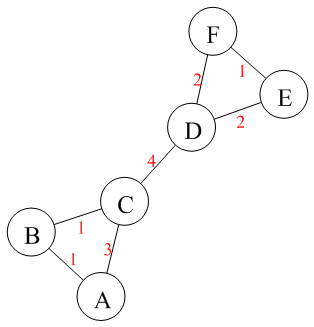
\includegraphics[height=8cm]{background/background-partitionhierarchies-pathfinding-transitiontable-a.png}}%
	%
	\hspace{4mm}%
	%
	\subfigure[]
	{
	\raisebox{1cm}{\begin{tabular}[b]{cc|cccccc}
	&& \multicolumn{6}{c}{Destination} \\
	&& A & B & C & D & E & F \\
	\hline
	\multirow{6}{*}{Source}
	& A  & $\times$ & B & B & B & B & B \\
	& B  & A & $\times$ & C & C & C & C \\
	& C  & B & B & $\times$ & D & D & D \\
	& D  & C & C & C & $\times$ & E & F \\
	& E  & D & D & D & D & $\times$ & F \\
	& F  & D & D & D & D & E & $\times$
	\end{tabular}}
	}%
\caption{A graph and its corresponding transition table -- each table entry $t_{SD}$ stores the node after $S$ on the optimal path between $S$ and $D$}
\label{fig:background-partitionhierarchies-pathfinding-transitiontable}
\end{stusubfig}
%---

Hierarchical pathfinding is an approach designed to reduce these prohibitive storage costs. The essence of the idea is to partition the graph into clusters. This partitioning of the graph into clusters creates a two-layer partition hierarchy (in this case a partition forest) of the graph nodes. Pathfinding schemes can then be devised that still produce optimal paths, but only store the substantially smaller transition tables for paths within each cluster and a transition table for an inter-cluster `super-graph' -- for an illustration of this sort of scheme, see Figure~\ref{fig:background-partitionhierarchies-pathfinding-kim}. The kind of storage savings that can be expected from this sort of approach are quantified by Dickheiser in \cite{dickheiser04}.

%---
\stufigex{height=11cm}{background/background-partitionhierarchies-pathfinding-kim.png}{Partitioning a large graph into clusters allows us to only store transition tables for each cluster (b) and the super-graph (c), rather than a transition table for the entire graph. When finding paths, all the necessary information is contained in the transition tables for the source cluster, the destination cluster and the super-graph (d). (The figure is reproduced from Kim et al.\ \cite{kim98}.)}{fig:background-partitionhierarchies-pathfinding-kim}{p}
%---

To find an optimal path between two nodes using this scheme, we observe that such a route can either (a) go from the source node to a boundary node of the source cluster, then (via the super-graph) to a boundary node of the destination cluster, then to the destination node, or (b) go directly from the source node to the destination node if they are in the same cluster. (Note that the shortest path between two nodes in the same cluster may actually go via the super-graph, so we have to consider both options in such a case.) An optimal intra-cluster route (where applicable) can simply be looked up in the cluster's transition table, but to find an optimal inter-cluster route is slightly more involved. To do so, we find three sets of optimal sub-paths:
%
\begin{enumerate}

\item $S = \{s_i\}$, the set of optimal paths from the source node to a boundary node of the source cluster. These can be looked up using the source cluster's transition table.
\item $P = \{p_j\}$, the set of optimal paths from a boundary node of the source cluster to a boundary node of the destination cluster. These can be looked up using the super-graph's transition table.
\item $D = \{d_k\}$, the set of optimal paths from a boundary node of the destination cluster to the boundary node. These can be looked up using the destination cluster's transition table.

\end{enumerate}
%
We then consider all possible paths $s_i \mbox{++} p_j \mbox{++} d_k$ (where $\mbox{++}$ represents path concatenation) and pick one with the lowest cost. This is minimised against any possible intra-cluster route where necessary to give a path that is optimal overall.

Thus far, we have only considered a pathfinding hierarchy with two layers, but the scheme can easily be extended to allow more layers if e.g.~the transition tables for the individual clusters are still considered too memory-intensive. The easiest way to do this is to treat each individual cluster as a graph in its own right and partition it into pieces (a top-down approach), although bottom-up approaches are also possible (one such approach, referred to in \cite{kim98}, can be found in \cite{jing96}). Actually constructing the partitions of individual graphs automatically is the problem known as graph partitioning or graph clustering (see e.g.~\cite{huang96,jing98}, or indeed \S\ref{subsec:graphpartitioning}). In certain domains (such as the computer games industry), the partitions may actually be constructed manually to gain finer control over the end result \cite{dickheiser04}. In either case, however, it is helpful to be able to edit the resulting partition forest interactively to try and minimise the amount of memory required to store the transition tables. This can be facilitated by the partition forest algorithms I will present in Chapter~\ref{chap:ipfs}.

\subsection{Team Organisation}

TODO

\subsection{World Representation}

TODO: \cite{finkel74,fuchs80}

%---
\section{Chapter Summary}

This chapter has given an overview of most of the techniques currently in use for medical image segmentation and provided some important background on the varied uses of partition hierarchies. In Chapter~\ref{chap:methodology}, I will discuss the design of my research in the context of these large bodies of existing work.

\chapter{Background}
\label{chap:background}

\emph{Draft Version}

%---
\section{Segmentation}

\subsection{Introduction}

Segmentation is a sub-field of image processing in which we try to partition an image into regions which correspond to interesting, or salient, features in the image. For instance, in medical image processing, we might try and segment a CT scan into regions which correspond to axial slices through major organs, e.g. the liver or a kidney. Segmentation is rarely useful on its own; rather, it tends to occur as a pre-processing step whose output (the partition of the image) is then used as input to later stages of an algorithm. An example usage is in the 3D visualization of organs, where the segmentation results for a series of slices can be used to identify which voxels in a volumetric dataset are contained within a given organ: a mesh can then be generated from this using any suitable algorithm from the visualization literature, e.g. \cite{cong05,lorensen87,wu03}.

Many different approaches are used to segment images. There is no `best' method which works well for every segmentation problem, so it is vital to select a method carefully based on the characteristics of the images under consideration. Since I will be dealing exclusively with \emph{medical} image segmentation of abdominal scans for the purposes of my thesis, I will only discuss techniques applicable in that domain in this review, but even with that restriction in place, there are several different image modalities (e.g. CT, MRI, US) which may be encountered and a large number of different segmentation methods in use \cite{pham00,varshney02}.

Each segmentation algorithm has its own characteristics (e.g. resilience to noise, connectedness of output, etc.), making it more or less suitable for a given problem. Some algorithms output region boundaries (contours) rather than an actual partition of the image \cite{kass88,lobregt95,xu98}: this may or may not be desirable in a given context (although it is worth noting that is often possible to subsequently convert between region-based and boundary-based representations). Furthermore, the degree of automation of the algorithms varies. At one end of the spectrum, images can be manually segmented by a radiologist: this generally gives excellent results (although they may not necessarily be entirely consistent between different radiologists) but requires more human interaction, although radiologists have got this down to a fine art. At the other extreme, we can try and develop algorithms which segment images automatically \cite{lee03, lin06, marcotegui05, meijster98, park03, soler01, touhami05, tsagaan02}: these reduce the burden on the human user, but it is rare that results are attained which are comparable with those which can be produced manually, not least because radiologists sometimes have to rely on anatomically-informed judgement to decide where the boundary of an object of interest lies and it is difficult to incorporate this expert knowledge into a computer program. That being said, some teams have achieved exceptionally good results in this area. Of particular note is the work done by Luc Soler's team in France \cite{soler01} which aims to delineate anatomical structures relevant to hepatic surgery. Clinical validation on over 30 patients has shown that their fully-automatic segmentation technique on 2mm-thick enhanced spiral abdominal CT scans generates results which are often actually \emph{better} than the manual segmentation produced by a radiologist.

In general, though, some degree of interactivity in segmentation procedures currently remains desirable, whether this merely involves allowing a radiologist to make adjustments to the output, or actually involves requesting user input to the algorithm itself (for example, a region growing algorithm might require seed points). There is a lot of overlap between the methods used for fully-automatic and semi-automatic segmentation --- in general, fully-automatic segmentation tends to focus (not surprisingly) on automating the difficult-to-automate aspects of semi-automatic algorithms --- so I will review approaches from both sub-fields in the following sections.

\subsection{Thresholding}

%TODO: \cite{kobashi95,seo05}

%In principle, thresholding segmentation methods are quite simple. The idea is to divide the pixels of the image into two (in the case of binary thresholding) or more (in the case of multithresholding) classes through the use of one or more dividing lines on the image histogram. For example, in an 8-bit image where the grey levels ranged from 0 (black) to 255 (white), we could decide that all pixels whose grey value was greater than 160 (say) represented the foreground of the image, and all other pixels represented the background.

In principle, thresholding segmentation methods are quite simple. The idea is to divide the pixels of the image into classes through the use of one or more dividing lines on the image histogram. Dividing the image into two classes is known as \emph{binary thresholding}; where more classes are used, we refer to the process as \emph{multi-thresholding}. As an example, we could use binary thresholding to divide an 8-bit image (with grey levels ranging from 0=black to 255=white) into two classes, one containing pixels greater than (say) 160, and representing the foreground of the image, and the other containing all the remaining pixels and representing the background.

The difficulty encountered in practice is how to determine the optimum threshold location(s). A misplaced threshold will cause an inaccurate segmentation, so choosing the location appropriately is essential. In our example above, choosing a threshold which was too high would mean that the foreground of the image would be \emph{undersegmented} (i.e. pixels which should be classified as being part of the foreground are incorrectly classified as background) and the background would be \emph{oversegmented} (the converse). Choosing too low a threshold would cause the opposite problem.

Owing to difficulties like this, applications are often designed so that thresholds can be chosen interactively by the user, but a great deal of work has also been done on automatically determining good threshold locations. As surveyed in \cite{sezgin04}, there are six types of approach to the problem in current use, including:

\begin{enumerate}

\item \emph{Histogram shape-based methods.} These use shape properties of the histogram to find a good threshold. For instance, Rosenfeld's histogram concavity method, cited in \cite{lee.c92}, works by examining the difference between a histogram and its convex hull. A grey level at which the the height difference between the histogram and its convex hull is greatest (i.e. a point of deepest concavity) is picked as the threshold value.

\item \emph{Clustering-based methods.} These try and group the grey level data into a given number of clusters (two in the case of binary thresholding). One example is the method of Ridler and Calvard \cite{ridler78}. Their idea was to take a grey-level image and produce an initial binary classification which makes the assumption that the object of interest is somewhere in the middle of the image and the corners of the image contain only background. The means of the pixels currently classified as background and object are calculated and the average of the two means is taken. The new value is then used to threshold the image and produce a new binary classification into background and object classes: it is assumed that this will be more accurate than the initial guess. Finally, the process is iterated until there is little or no change in the binary classification, and the last threshold in the iteration is chosen for use.

\item \emph{Entropy-based methods.} These are based on information theory and pick thresholds by (for example) trying to maximise the information content in the thresholded image. As described in \cite{wong89}, the simplest possible method looks at two probabilities, $F(T)$ and $F^*(T) = 1 - F(T)$, each parameterised in terms of a threshold, $T$. The first, $F(T)$, gives us the probability of a given pixel having a grey value less than or equal to the threshold, and the second, $F^*(T)$, gives us the probability of the value being greater than it. The information content in the thresholded image is given by
%
\[
H(T) = -F(T) \log_2 F(T) - F^*(T) \log_2 F^*(T)
\]
%
and attains a maximum when $F(T) = 0.5$. This is equivalent to saying that in the absence of any other knowledge, the maximum entropy principle tells us that the information contained in the thresholded image is maximised by picking a threshold which classifies half the pixels as background and half as foreground. This makes intuitive sense, but is too simplistic an approach for the majority of applications. Better alternatives have been developed, but are beyond the scope of this report.

%\item \emph{Object attribute-based methods.}

%\item \emph{Spatial methods.}

%\item \emph{Local / adaptive methods.}

\end{enumerate}

\noindent In spite of the large amount of work done on thresholding, however, it has some significant downsides when used on its own to process medical images:

\begin{itemize}

\item It divides the image into two or more groups of pixels, based on their grey values, but there is no guarantee (or even an expectation) that any of these groups will be contiguous in the image. For instance, trying to segment a kidney from a CT scan by bounding it between two grey value thresholds might also result in inadvertently segmenting blood vessels across the image as well (their grey levels are quite similar to those of the kidneys). Not only are these blood vessels not part of the kidney, they are actually physically separated from it in the image! (It is also worth noting that trying to segment a kidney will generally result in segmenting both of them at once, since their grey level ranges are the same. This sort of problem can be overcome by specifying the side of the body in which we're interested.)

\item It is by no means the case that acceptable threshold locations always exist. If the grey value ranges of different objects of interest significantly overlap, it may be impossible to separate them using thresholding alone.

\end{itemize}

%For reasons like this, I believe that thresholding is not the most appropriate choice of method for my work. However, I have found a use for it when trying to quantify the extent of necrosis in a tumour (see Chapter~\ref{chapter:existingwork}).% Whilst it is true that thresholding can be made to produce reasonable results (e.g. \cite{kobashi95}), I feel that there are other algorithms which

These limitations can often be overcome by combining thresholding with other techniques. For instance, the results of thresholding often have gaps in them, which can sometimes be filled in by carefully applying various morphological operators (e.g. morphological opening and closing). Luc Soler's team \cite{soler01} made use of thresholding (as one technique among many) and achieved excellent automatic segmentation results for the liver. However, they did not use thresholding on its own. For instance, they segmented bones by thresholding for bright areas and then keeping only those which were near to the fat tissue (which had already been segmented). Simple thresholding alone would have been insufficient for the task, since structures such as the aorta also appeared bright on the contrast-enhanced images.

%Whilst thresholding has its limitations, it has been nevertheless been successfully incorporated into more general segmentation algorithms, sometimes with spectacularly good results. The work of Luc Soler's team \cite{soler01}, as previously commented on, is particularly noteworthy in this regard. One example of how they use thresholding to achieve good results is when they are segmenting bones. A simple thresholding operation would fail, since the contrast agent used when the scans were taken causes structures such as the aorta to appear bright. Instead, they isolate the fat tissue and define the bones as being bright structures close to that. They also post-process their thresholding operations with morphological operators to fill in any unwanted gaps.

\subsection{Region Growing}

%TODO: \cite{lin06,pohle01}

Region growing methods for segmentation essentially work as follows. First, an initial seed point is chosen for a feature of interest. Then, the region is `grown' by iteratively considering all points which are adjacent to the region and adding any which satisfy certain criteria. For example, we could choose to add adjacent pixels whose grey value differs from that of their neighbour in the region by less than a certain amount. Alternatively, we could try and add adjacent pixels which preserve the homogeneity of the entire region (for some suitable definition of homogeneity). A basic region growing algorithm can be implemented straightforwardly using a queue. Starting from a queue containing only the initial seed point, we repeatedly pop the pixel at the front of the queue, consider its non-region neighbours for addition to the region, and push any which satisfy the requisite criteria onto the end of the queue. The process terminates when the queue empties.

The key issues when implementing region growing are how to choose the seed point, how to formulate the criteria specifying which points to add to the region, and how to decide when the process should terminate. For automated segmentation methods, how to choose the seed point is of fundamental importance; semi-automated algorithms can focus exclusively on the latter two problems, relying instead on the user to interactively specify an initial seed.

As mentioned above, one of the simplest approaches to region growing is to add adjacent pixels which are within a certain fixed threshold value of their neighbour in the region. Practical region growing methods, however, such as \cite{lin06,pohle01}, tend instead to use \emph{adaptive} region growing, whereby the criterion varies to take account of the area around the pixel under consideration. In \cite{lin06}, for example, the approach taken is as follows. After locating an initial seed point $(s_x, s_y)$, a $7 \times 7$ mesh is placed over it and the maximum and minimum pixel intensities within the mesh, $M(s_x, s_y)$ and $m(s_x, s_y)$ are determined. From these, a contrast range $t_0 = M(s_x, s_y) - m(s_x, s_y)$ is calculated and recorded. Next, for each pixel $(x,y)$ under consideration for addition to the region, values $M(x,y)$ and $m(x,y)$ are similarly calculated, and a local value $\theta_{\rm local} = (M(x,y) + m(x,y)) / 2$ is determined. The region growing criterion is then formulated as $|f(x,y) - \theta_{\rm local}| \le t_0$, i.e. we add an adjacent pixel $(x,y)$ to the region if the absolute difference between its grey value $f(x,y)$ and the midpoint of the contrast range of the $7 \times 7$ mesh surrounding it is less than the contrast range of the $7 \times 7$ mesh centred on the initial seed point. The region growing is specified to stop when this absolute difference is greater than a certain threshold, implying that the area surrounding a given pixel is not homogeneous.

The advantages of region growing methods are that the resultant region is guaranteed to be connected in the image (unlike with thresholding) and that they are, on the whole, fairly easy to implement. However, from the point of view of automatic segmentation, they present difficulties, because choosing an initial seed point is in general a non-trivial problem. The usual approach taken for automatic seed point selection is to rely on statistical data about where the features of interest (e.g. organs) usually lie in the body. For instance, the approach in \cite{lin06} is to search for suitable seed points in two elliptical regions on each side of the body, one for each kidney. This works quite well, but doesn't seem as if it would be that robust if tested on unusual cases.

Whilst region growing algorithms are guaranteed to produce a connected result, the region may still have holes in the middle of it. Whilst this may be desirable if we really are trying to segment a torus-shaped feature, on the whole we need to post-process the region growing results to remove these holes. Common techniques for doing this include morphological closing, etc.

\subsection{Approaches from Mathematical Morphology}

In the words of some of its practitioners\footnotemark{}, the field of mathematical morphology espouses a `non-linear approach to image processing'. Its interesting techniques include dilation, erosion, and morphological opening and closing, but our emphasis in this report will be on one particularly useful morphological technique for image segmentation: the watershed transform.

\footnotetext{The Centre for Mathematical Morphology at the Ecole des Mines de Paris.}

\subsubsection*{The Watershed Transform: Techniques}

%TODO: \cite{bieniek00,meijster98,osma-ruiz06,rambabu07,stoev00}

\emph{Note: I have written an article on the watershed transform for ACCU's Overload journal, which appears as Appendix~\ref{chapter:watershed} in this report. For that reason, I plan to give only a limited presentation of the technique here. Readers are referred to the appendix for more information.}

The idea of the watershed transform is to view an image as a landscape and divide it up into valleys. Each valley in the landscape will correspond to a region in the segmentation result. We don't perform the transform on the actual image to be segmented, since its valleys may not correspond to the features we're interested in. Instead, we take the initial image and try and generate a derived image from it in which the valleys correspond to our features of interest: in the case of medical images, this often involves something similar to taking the gradient of the initial image, since organs tend to look fairly homogeneous on scans (and thus the magnitude of the gradient within them is low). The derived image then becomes the input to the watershed transform itself.

In terms of implementation, the watershed transform can be viewed in one of two different ways:

\begin{enumerate}

\item \emph{A flooding/immersion process}. Imagine poking holes in the local minima of the landscape and then lowering the landscape vertically into a lake. As the landscape is lowered, water will seep through the holes and catchment basins will form in each of the valleys of the image. As the water continues to rise, some of the catchment basins will meet: at this point, we add dams, or watersheds, to keep them apart, and continue lowering the landscape. At the end of the process, the dams we added will act as dividing lines between the valleys, thus segmenting the underlying image into regions.

\item \emph{A rainfall process}. Imagine dropping a raindrop at each point in the landscape. Assuming the image has no (non-minimal) plateaux (flat regions), the drop will run downhill, via a path of steepest descent, until it ends up in a local minimum. (There are ways of dealing with non-minimal plateaux, e.g. the method described in the appendix.) The point at which it started will be associated with this local minimum (it will be called part of the minimum's catchment basin) and the process will continue until all the points in the landscape have been processed. The result will be a region-based partition of the landscape (and hence the underlying image) into catchment basins, one per local minimum.

\end{enumerate}

These two alternative ways of viewing the process have led to two different classes of techniques. In particular, \cite{bieniek00} and \cite{rambabu07} are examples of the former approach, and examples of the latter can be found in \cite{meijster98,osma-ruiz06,stoev00}. It is worth noting that the various definitions are not always exactly equivalent. For example, some approaches generate results containing watershed lines, whilst others generate only regions. Also, rainfalling approaches don't generally give identical results to their immersion-based counterparts. It is thus important to choose an appropriate method with care.

\subsubsection*{The Watershed Transform: Pre-Processing}

%TODO: \cite{ancin95}

The biggest problem with the watershed transform as a segmentation approach is that it is overly affected by spurious local minima in the landscape. This leads to massive over-segmentation of the image. To explain the problem, consider an analogy. If we try and divide a dimpled landscape into valleys, counting each dimple (small hollow) in the landscape as a valley, then we will end up with vast numbers of `irrelevant' valleys at the end of the process, obscuring the more significant valleys we are trying to find: this is essentially the problem faced by the watershed transform. The `dimples' in an image can be caused by things like noise, but even in the absence of image artifacts, there will usually be valleys corresponding to features in which we have no interest. We need a way of separating the wheat from the chaff.

To overcome this difficulty, various approaches have been suggested in the literature. The effects of less prominent noise can be mitigated to an extent by smoothing the image, although care must be taken not to blur the edges in the image when doing this. Another approach \cite{ancin95} is to suppress some of the irrelevant contours in the gradient image by determining the connected components of the gradient image and removing (by setting the pixels of the component to zero) all those whose size is less than a threshold (e.g. the perimeter of the smallest object of interest).

One technique which works quite well in practice is to apply spatially-variant smoothing to the image: instead of smoothing uniformly over the entire image, the idea is to smooth less in areas where we think there may be edges. This is the idea behind non-linear diffusion filters \cite{perona90}. (In Chapter~\ref{chapter:existingwork}, I describe another approach based on similar principles.)

\subsubsection*{The Watershed Transform: Post-Processing}

%TODO: \cite{beucher01,patino05,marcotegui05,wegner95}, \cite{najman96} (mention correction paper)

The approaches described so far try to pre-process an image (or its gradient image) to reduce watershed over-segmentation. Post-processing the watershed results is also possible, and in general a combination of both techniques tends to be employed.

The general idea of watershed post-processing is to try and merge the large number of generated regions together in a way that generates larger regions corresponding to our objects of interest. Attempts can be made to group together similar regions using fuzzy relations, e.g. \cite{patino05}.

The idea of region-merging can also be used to create partition hierarchies, intuitively corresponding to a series of segmentations of an image at different scales. For example, the waterfall algorithm \cite{beucher01,marcotegui05} merges regions by iteratively running a watershed-from-markers algorithm on the region adjacency graph of the watershed result. (Note that I have described it in much more detail in Appendix~\ref{chapter:waterfall}.) This is particularly useful when trying to pick out organs of different sizes. A similar approach is described in \cite{wegner95}.

The type of hierarchy generated by the waterfall algorithm is by no means the only possible hierarchy, and indeed it may converge (to a single region) too fast for some applications. Alternative hierarchies are also possible, e.g. ones based on the saliency of contours in the watershed results \cite{najman96}.\footnotemark{}

\footnotetext{Whilst this is generally a good paper, it is worth noting that it contained an error which had to be corrected later in a comment \cite{lemarechal98}. An improved correction was then published by one of the original authors \cite{schmitt98}. All three should be read together to avoid confusion.}

%\subsubsection*{The Watershed Transform: Applications}

%TODO: \cite{bueno01,grau04}, mention \cite{najman95} in the context of registration

\subsection{Deformable Models}

%Model fitting methods, as their name suggests, attempt to fit a model of the features under consideration to the actual data available. They essentially make use of \emph{a priori} anatomical knowledge at an early stage of the segmentation process to improve the generated results. The actual model used can take a variety of different forms, ranging from deformable models, whereby the model is represented explicitly (perhaps as a contour on the image), to implicit model representations such as probabilistic atlases and neural networks. I will briefly survey each of these methods in the subsections which follow.

%As their name suggests, deformable models methods work by taking an initial model of the features under consideration and deforming it to fit the actual data available. The initialisation of the model is generally based on \emph{a priori} anatomical knowledge. As observed in \cite{suri02}, there are two basic types of deformable model, namely \emph{parametric} and \emph{geometric}. Geometric deformable models have been developed more recently than their parametric counterparts, but both types see a lot of use. The most well-known examples of the two types are snakes and level sets, which will be discussed in detail in the following two subsections.

As their name suggests, deformable models methods work by taking an initial model of the features under consideration and deforming it to fit the actual data available. The initialisation of the model is generally based on \emph{a priori} anatomical knowledge. The model itself can be represented in a variety of ways, and these ways correspond to a number of different approaches to the problem. For example, the snakes method, which we will see shortly, represents the model as a parametrically-defined spline, and is hence referred to as an example of a parametric deformable model (it is sometimes also referred to as an explicit deformable model). In contrast, level sets represent the model \emph{implicitly} and are an example of implicit deformable models. Implicit deformable models were developed more recently than their parametric counterparts, but both types see a lot of use.

\subsubsection{Snakes}

%TODO: \cite{cohen91,kass88,lobregt95,xu98}

As originally defined by Kass, Witkin and Terzopoulos in \cite{kass88}, ``A snake is an energy-minimizing spline guided by external constraint forces and influenced by image forces that pull it toward features such as lines and edges.''

Essentially, the idea works as follows. We represent the position of the snake, in terms of a spline parameter $s$, as $\mathbf{v}(s) = (x(s),y(s))$, and define an \emph{energy functional}, $E_{snake}^*$, as
%
\[
E_{snake}^* = \int_0^1 E_{int}(\mathbf{v}(s)) + E_{image}(\mathbf{v}(s)) + E_{con}(\mathbf{v}(s)) \; ds.
\]
%
The three terms in the summation are \emph{internal} energy, which tries to limit the curvature of the snake, \emph{image} energy, which tries to attract the snake towards features in the image such as lines and edges, and \emph{constraint} energy, which allows the user to apply constraints to influence the result of the segmentation. The snake algorithm as a whole attempts to find a spline minimising $E_{snake}^*$.

The original snakes paper describes a continuous model, but more recent research \cite{lobregt95,miller90b,miller90a} has seen the development of discrete models as well. The model described by Lobregt and Viergever in \cite{lobregt95}, called a \emph{discrete dynamic contour model}, is particularly interesting, both because it is intuitively easy to understand, and because it links in with my previous work. It is thus worth describing in more detail.

Rather than relying on ideas of energy-minimization, Lobregt and Viergever model snakes using a force-based physical simulation (note that this ties in well with my earlier work on physical simulations of long hair \cite{gvc08}). In their approach, a snake is a set of vertices connected by edges. At each time-step, various forces are applied to each vertex, which gradually \emph{deform} the snake towards the desired result. The results of this approach will depend to an extent on the lengths of the edges joining the vertices: if an edge is too long, important image features may pass through the gaps between vertices; if it is too short, the snake may become overly fixated on small details, not to mention the speed of the process being adversely affected. For this reason, after each deformation step, the snake is \emph{resampled} (by adding or removing vertices where necessary) to keep the edge lengths within certain limits.

The forces applied to each vertex closely mimic the energy terms in the original snakes paper. The force $\mathbf{f_i}$ applied to vertex $i$ is defined as the weighted sum
%
\[
\mathbf{f_i} = w_{ex}\mathbf{f_{ex,r_i}} + w_{in}\mathbf{f_{in,i}} + \underbrace{w_{damp}}_{< \; 0}\mathbf{v_i},
\]
%
where $\mathbf{f_{ex,r_i}}$ is an \emph{external} force term corresponding to the image and constraint terms from the original formulation, $\mathbf{f_{in,i}}$ is an \emph{internal} force term corresponding to the original internal term, and the remaining term is a new addition used to apply damping to try and bring the simulation to rest. (The real numbers $w_{ex}$, $w_{in}$ and $w_{damp}$ specify the weights to be given to each of these three factors. The paper tended to set all three of these to $0.5$: apparently this was derived empirically.)

It is important to mention that the method relies on quite a close initialisation (i.e.\ image features have quite a short capture range). In \cite{ree05}, this problem is circumvented by peforming a watershed-from-markers segmentation and using the result of that to initialise the snake. Another alternative, referred to there, is to try and add additional external forces to solve the problem: in particular, some success has been had with \emph{balloon forces} \cite{cohen91} and \emph{gradient vector flow} \cite{xu98}.

Problems of this kind with snakes methods have led to a great deal of interest in level sets as an alternative, although snakes also remain popular as a well-established and far simpler alternative. They also have the advantage that they can represent open structures as well as closed ones.

\subsubsection{Level Sets}

%TODO: \cite{sorlie05}

Level sets are to snakes what implicit representations of functions are to parametric ones. As an initial introduction, consider the alternative representations of a circle of radius $r$, centred at the origin. An implicit representation could be
%
\[
x^2 + y^2 = r^2,
\]
%
whereas a parametric representation in terms of an angle $\theta$ could be
%
\begin{eqnarray*}
x & = & \cos \theta \\
y & = & \sin \theta.
\end{eqnarray*}
%
Now, consider a more general form of the above. Instead of thinking about circles, consider the function $\phi(x,y) = x^2 + y^2$, which defines a scalar field over $\mathbb{R}^2$. For any value $k > 0$, the equation $\phi(x,y) = k$ defines a circle in the x-y plane: we will refer to each of these circles as an \emph{isosurface} of $\phi$, because each of them is the surface (curve) of all the points at which $\phi$ takes a particular value\footnotemark{}.

\footnotetext{\emph{Iso} means `equal' in Greek, so here we are talking about the surface containing all the points with the same $\phi$ value.}

Note what happens if we change $\phi$. If we redefine it as $\phi(x,y) = x^3 + y^3$, the isosurfaces change from being circles to hypercircles. This is a key idea: by changing the function $\phi$, we can move the isosurfaces of $\phi$ around, \emph{without having to represent them explicitly}. This is the insight behind level sets: we represent the contour we're interested in as an isosurface of some function $\phi$, then modify $\phi$ to modify the contour. Instead of using simple functions like $x^2 + y^2$ for our $\phi$, we can think of a general function $\phi: U \to \mathbb{R}$, where $U \subset \mathbb{R}^2$.

In practice, to represent contour changes over time, we make $\phi$ a function of time as well, giving us $\phi(\mathbf{x},t): U \times \mathbb{R}^+ \to \mathbb{R}$. We then set this equal to some constant $k$ to actually specify which isosurface of $\phi$ we're interested in.

Consider a simple example, that of a circle, centred at the origin, which gradually expands outwards as the time increases (see Figure~\ref{fig:levelsets-circle}).

%---
\stufigex{height=7cm}{background/levelsets-circle.png}{A simple circular contour which gradually expands over time}{fig:levelsets-circle}{H}
%---

In particular, suppose its radius is $t$ at time $t$. We represent this as:
%
\[
\phi((x,y), t) = \frac{x^2 + y^2}{t^2} = 1 = k
\]
%

For a more complicated example, consider gradually changing the circle into an ellipse over time (see Figure~\ref{fig:levelsets-ellipse}).

%---
\stufigex{height=7cm}{background/levelsets-ellipse.png}{An example of a contour which changes its shape over time}{fig:levelsets-ellipse}{H}
%---

This could be achieved by writing the following:
%
\[
\phi((x,y), t) = \left(\frac{x}{t}\right)^2 + y^2 = 1 = k
\]
%

In practice, we are almost never able to give an explicit function for $\phi$: the simple examples above notwithstanding, it's just not possible for real-world applications. Instead, we discretise the process by specifying initial values for $\phi$ at points on a discrete grid, then derive a partial differential equation for $\phi$ and solve it numerically to modify the contour over time. The PDE in question can be found by taking the total derivative of
%
\[
\phi(\mathbf{x}, t) = k,
\]
%
giving us
%
\[
\pd{\phi}{t} = -\nabla\phi \cdot \mathbf{v},
\]
%
where $\mathbf{v} = \pdnf{\mathbf{x}}{t}$. By making $\mathbf{v}$ a function of the position of $\mathbf{x}$ and the geometry of the surface (which it turns out can be represented by the differential structure of $\phi$), we can control how we want the contour to evolve over time.

How to numerically solve the above equation is beyond the scope of this report, but before moving on, I would like to look at a concrete example of the method on a discrete grid, to illustrate some of its advantages. Consider the discrete grid of $\phi$ values in Figure~\ref{fig:levelsets-discrete1}(a). The marked points form an isosurface of $\phi$, specifically the $k = 4$ isosurface. This is entirely analogous to the examples above, but on a discrete grid instead of in a continous space. By changing the grid values, as in Figure~\ref{fig:levelsets-discrete1}(b), we can move the isosurface however we wish.

%---
\begin{figure}[H]
\begin{center}
	\subfigure[]{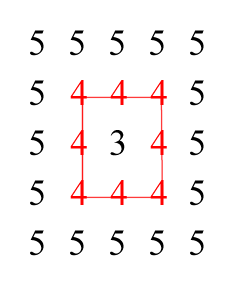
\includegraphics[height=5cm]{background/levelsets-discrete1a.png}}%
	\hspace{4mm}%
	\subfigure[]{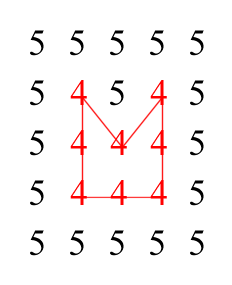
\includegraphics[height=5cm]{background/levelsets-discrete1b.png}}
\end{center}
\caption{An example of level sets on a discrete grid}
\label{fig:levelsets-discrete1}
\end{figure}
%---

Now, consider the further example shown in Figure~\ref{fig:levelsets-discrete2}(a). Here the situation seems more complicated, in that the points on the $k = 4$ isosurface are not all connected to each other. This is actually an advantage of the level set method, however. By representing the surface implicitly, we can model surfaces with multiple connected components without having to do any additional work. Indeed, the number of components can evolve over time: in Figure~\ref{fig:levelsets-discrete2}(b), we see that the two components can be joined by simply changing the value of $\phi$ at one of the grid points to $5$.

%---
\begin{figure}[H]
\begin{center}
	\subfigure[]{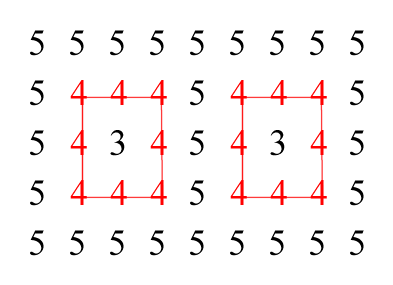
\includegraphics[height=5cm]{background/levelsets-discrete2a.png}}%
	\hspace{4mm}%
	\subfigure[]{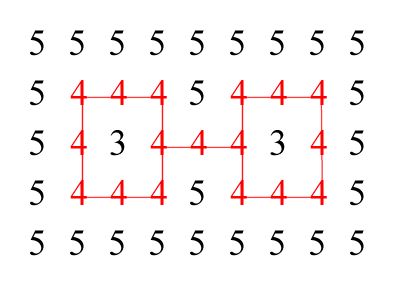
\includegraphics[height=5cm]{background/levelsets-discrete2b.png}}
\end{center}
\caption{An example with more than one connected component}
\label{fig:levelsets-discrete2}
\end{figure}
%---

One final advantage of level sets worth mentioning is that the method works equally well in 3D, although the extra processing involved means that clever numerical techniques are required. The details of how these work are beyond the scope of this report but, as an example, one method (the narrow-band technique) basically restricts numerical calculations to a narrow region around the isosurface we're particularly interested in. The insight is that solving the PDE over the whole domain is only necessary if we're interested in solving for the entire family of isosurfaces associated with $\phi$: often we're only looking at a single isosurface, so the extra computations aren't necessary. For more details, take a look at \cite{yoo04}.

\subsubsection{Other Deformable Models}

%TODO: \cite{jalba04,rao05,tsagaan02}

Other notable parametric deformable models in existence include the contribution of Tsagaan et al. \cite{tsagaan02}, who used a NURBS-based model of a kidney and deformed it by minimising an energy function. Their results seem good in some cases, but differ markedly from the manually segmented results in others.

Parametric and implicit models are not the only types of deformable model in use, however. In particular, \cite{jalba04} uses a deformable model based on charged particles to achieve some interesting automatic segmentation results. Here, the model is represented as a set of charged particles under the influence of an electrostatic field. The authors' work in this area is still ongoing. Yet another deformable model can be found in \cite{pizer03}, in which the authors' make use of a medial representation known as m-reps.

\subsection{Learning Methods}

Learning segmentation methods generally start with a training phase, in which a large number of scans are taken and used to construct some variety of model, which encodes information that can be used to segment subsequent scans. Two different types of learning method will be discussed in the following subsections.

\subsubsection{Atlas-Based Approaches}

%TODO: \cite{park03,zhou05}

Atlas-based methods start by constructing an atlas, or reference segmentation, from a set of training data. For instance, in \cite{park03}, a probabilistic atlas was constructed by registering (aligning) the manually segmented volumes of 31 patients onto that of a carefully chosen reference patient (thus the data came from 32 patients in all). The atlas was represented as a 3D grid of vector values, where the components of each vector corresponded to the organs under consideration, and the values of the components indicated the fractional percentage of registered data sets in which the point was labelled as the given organ. As an example, if we were considering the liver and the two kidneys, the vector $(0.4, 0.6, 0)^T$ at a point could indicate that the point was inside the liver in 40\% of the data sets and inside the right kidney in 60\% of them.

After constructing such an atlas, new sets of data can be segmented by registering them onto it. In \cite{park03}, they use a \emph{maximum a posteriori} (MAP) approach after registration to find the segmentation result which best explains the observed data. The important point here is that the segmentation result is based on both the data for the individual patient and the information encoded in the atlas. The atlas provides the prior probabilities at each voxel, and these are refined in light of the actual patient data.

To use the notation in \cite{park03}, we denote the segmentation result field as $\mathbf{X}$, the field of observed data for the individual patient as $\mathbf{Y}$, and the probabilistic atlas as $\mathbf{A}$. Each of these represents a volume of $N$ voxels, indexed linearly (in some order) from $1$ to $N$. So for instance, a particular segmentation result could be given by $\mathbf{x} = (x_1, x_2, \ldots, x_N)$. Our aim is to find the best possible $\mathbf{x}$, defined as
%
\[
\mathbf{\hat{x}} = \argmax_{\mathbf{x}} \mathbf{P}(\mathbf{X} = \mathbf{x} | \mathbf{Y} = \mathbf{y}).
\]
%
In other words, we seek the segmentation result which best explains the observed patient data, $\mathbf{y}$. The probabilistic atlas is used in all of this as the prior for $\mathbf{X}$. Suppose there are $L$ different possible voxel labels, numbered from $1$ to $L$. Each voxel $a_i$ of the probabilistic atlas contains an $L$-vector, $(a_{i,1}, \ldots, a_{i,L})$, where $a_{i,\ell}$ gives the probability of a voxel's correct label being $\ell$. We use this to define the prior probabilities for $\mathbf{X}$, writing
%
\[
P(x_i = \ell) = a_{i,\ell}.
\]
%
In other words, the probability of the correct segmentation result for a given voxel being $\ell$ is given by the $\ell^{th}$ component of the probabilistic atlas at that location. With this link made, the result determined will depend on both the atlas and the observed data.

\subsubsection{Neural Network Methods}

%TODO: \cite{lee03,tsai94}

Neural networks (NNs) can be used to segment images in a number of ways. A simple NN technique can be found in \cite{tsai94}, where the authors use a feed-forward network to classify each pixel into one of three classes (liver, boundary or non-liver) according to the grey-level histogram of the 7x7 region centred on the pixel. (In practice, they use a histogram with 16 grey levels instead of 256, to avoid a proliferation of input nodes in the NN.) The schematic of how this works (borrowed from their paper) is shown in Figure~\ref{fig:neuralnets-tsai}.

The NN is initially trained by picking a suitable image from the middle of the volume and marking a significant number of training regions for each class. The well-known back-propagation algorithm for NNs is used to update the weights on the network arcs accordingly.

The results of the scheme are somewhat hard to evaluate since the images in this somewhat old paper (1994) have not really survived the ravages of time. However, they do seem to show that the authors have obtained something that looks reasonably like a liver, so the method has some merit.

%---
\stufigex{height=20cm}{background/neuralnets-tsai.png}{Schematic diagram of the neural-network-based boundary detection method used in \cite{tsai94} (borrowed from the paper in question)}{fig:neuralnets-tsai}{H}
%---

\clearpage

A more up-to-date (and more complicated) NN scheme can be found in \cite{lee03}. Here, the authors use a multi-module, recurrent neural network to segment multiple abdominal organs (see Figure~\ref{fig:neuralnets-lee}). There is a module associated with each label under consideration. Each node of a given module $k$ corresponds to a pixel in the image and encodes the probability that the pixel should be assigned label $k$. The weights of the network arcs are initially derived from (for example) a correlation matrix containing the likelihoods of various labels occurring next to each other. (For example, the liver might be quite likely to occur next to the right kidney, but definitely shouldn't occur next to the left kidney.) An iterative state evolution algorithm is used to determine the probabilities at each node in each of the modules of the NN. The initial probabilities are generated using something called the `Kohonen self-organizing algorithm' (see the paper for details) and the nodes are updated at each time step based on the current probability at a given node and the support it receives from its neighbours. (So, for instance, if a pixel was currently classified as part of the left kidney, but all its neighbours were liver, it would be very likely to change to liver over time.) The results of this method (after combining it with fuzzy spatial rules for organ identification) are quite good (though the authors admit that more work is needed).

%---
\stufigex{height=8cm}{background/neuralnets-lee.png}{The architecture of the contextual neural network used in \cite{lee03} (borrowed from the paper in question)}{fig:neuralnets-lee}{ht}
%---

%\subsubsection{Statistical Methods}

%TODO: \cite{touhami05}

\subsection{Hybrid Methods}

%TODO: \cite{soler01}

It is often possible to achieve better results by combining a number of different segmentation methods than it is by using a single method on its own. A striking example of how successful this sort of technique can be is the work of Luc Soler's team in Strasbourg \cite{soler01} (see Figure~\ref{fig:soler} for a screenshot from their surgical tool).

%---
\stufigex{width=12cm}{background/soler.png}{An automatic 3D reconstruction of patients from medical images, as performed by the IRCAD surgical planning tools}{fig:soler}{t}
%---

The cited paper represents only a small part of their work on a surgical tool, and focuses on automatically segmenting the liver. Their segmentation method first uses thresholding, morphological operators and distance maps to identify the skin, bones, lungs, kidneys and spleen. The second stage is then effectively a clever deformable model approach in which they embed a reference model of the liver into the image and automatically deform it to the liver contours. Later stages use Gaussian fitting on the image histogram to separate normal liver tissue from blood vessels and lesions (tumours), a result which is further refined by their own analytical methods. The final stage of their work makes use of higher-level medical knowledge to label the hepatic portal vein and segment the liver anatomically: these features are not visible from the scans alone. As the screenshot shows, the results of this extensively hybrid technique are excellent.

Another couple of hybrid segmentation methods can be found in \cite{imielinska04}, in which the authors combine fuzzy connectedness, Voronoi diagram classification and deformable models into one segmentation method, and Gibbs priors and deformable models into another. The details of these techniques are beyond the scope of this report, but an implementation of the methods can be found in the popular (and freely-available) \emph{Insight Toolkit}.

\subsection{Evaluation of Segmentation Results}

%TODO: \cite{zhang96}

In many ways, evaluating the results of a segmentation process is just as important as segmenting the image in the first place. As described in \cite{zhang96}, there are essentially three different types of evaluation method in common use: analytical methods, empirical goodness methods and empirical discrepancy methods.

\emph{Analytical methods} deal with the actual algorithms rather than their results: they focus on things like the complexity of the algorithm, or its requirements. They usually produce qualitative results that are not directly tied to the segmentation accuracy for particular applications, which is often what we really want to know.

\emph{Empirical goodness} methods evaluate the segmentation results in terms of subjectively-defined `goodness' measures. For instance, some researchers have proposed methods which rate the results on their levels of intra-region uniformity (with high uniformity more desirable) and inter-region contrast (with high contrast more desirable). The advantage of using a method like this is that it can be applied directly to the segmentation results, without reference to any external source of information like a `gold standard' segmentation result. The disadvantage is that methods like this provide only subjective measures of segmentation quality.

In contrast, \emph{empirical discrepancy} methods compare the segmentation results to a `gold standard' result. This has the disadvantage of requiring us to have such a reference result (in the case of medical images, we may have to ask the radiologist to manually segment an image for us), but gives us a reasonably objective, quantitative evaluation of our algorithm in the context of a given application. One simple method in this category is to calculate the percentage of pixels misclassified. More complicated methods are also possible.

%---
\section{Region Classification / Organ Identification}

\iffalse

Aside from the segmentation process itself, a related problem is that of region \emph{classification}. This is the process of assigning \emph{meaning} to the regions we've identified. It ties in to segmentation in at least two ways: on the one hand, previously segmented regions can be classified into different categories (e.g. a given region could be classified as the liver); on the other, classification can be used to further refine a preliminary segmentation we've already obtained, perhaps by guiding a subsequent region-merging process (see my algorithm in Chapter~\ref{chapter:existingwork} for an example of this). In this way, performing segmentation and region classification in tandem, rather than consecutively, can help us obtain better results.

As noted in \cite{kobashi95}, designing positive shape constraints for organ identifaction is difficult as there are very few shape invariants. In other words, regions which should be classified as a given organ can come in a variety of different shapes. In contrast, \emph{negative} shape constraints, which specify shapes which a region \emph{cannot} take if it is to be classified as a given organ, are much more reliable and successful in this regard.

One paper which does deal with organ identification using positive shape constraints is \cite{lee03}, in which they use spatial fuzzy rules for organ recognition (the fuzziness helps them avoid some of the problems they would otherwise face by using positive shape constraints). Their rules were devised in collaboration with a radiologist. The results seem promising, but their method is not successful in all cases, as they admit themselves.

TODO: Read more papers on organ classification.

\fi

Region classification is the task of assigning \emph{meaning} to the regions identified by the segmentation process. As a clarifactory example, when we generate a kidney-shaped region, we're just doing segmentation, but when we identify it as a kidney we're doing region classification. The obvious way of classifying regions is to generate a series of useful properties for each region, and then use those to determine what the region might be. Useful properties might include location, area, mean grey value, elongatedness, etc. For instance, a feature which was located in the middle of the patient's back, appeared bright white on a CT scan and had an area of (say) $1000$ pixels or so might well be part of the spine.

In general, designing so-called \emph{positive} shape constraints like the above is difficult, as noted in \cite{kobashi95}, since there are very few shape invariants to rely upon. In other words, regions which should be classified as a given organ can come in a variety of different shapes. In contrast, \emph{negative} shape constraints, which specify shapes which a region \emph{cannot} take if it is to be classified as a given organ, can often be much more reliable and successful in this regard.

One paper which does deal with organ identification using positive shape constraints is \cite{lee03}, in which they use spatial fuzzy rules for organ recognition (the fuzziness helps them avoid some of the problems they would otherwise face by using positive shape constraints). Their rules were devised in collaboration with a radiologist. The results seem promising, but their method is not successful in all cases, as they admit themselves. Another relevant (if somewhat old) paper on this is \cite{cosic97}, in which they label CT scans of the head using rule-based labelling. However, it is hard to judge the quality of their results as the images are old and rather unclear.

Aside from methods involving shape constraints, it is also possible to classify regions based on their relative spatial relationships in the image \cite{atif07}. This is an interesting approach, because the spatial relationships between organs tend to exhibit much less variability than other properties such as the shapes of the organs in the images.


\chapter{Related Work}

TODO: Survey and critical assessment. Relation to own work.
\chapter{Analysis, design, implementation and interpretation of results}

TODO
\chapter{Critical Assessment}
\label{chap:assessment}

%##################################################################################################
\section{Chapter Overview}
%##################################################################################################

In Chapter~\ref{chap:introduction}, I listed six original contributions made by my doctoral work. Having now discussed the work underlying the contributions in detail in the preceding chapters, and validated my feature identification work in the previous chapter, the goal of this chapter is to evaluate the usefulness of these contributions both within the context of my doctorate and (where applicable) more widely.

%##################################################################################################
\section{Partition Forest Algorithms}
%##################################################################################################

In \S\ref{sec:ipfs-mutatingalgorithms}, I introduced a comprehensive set of algorithms for editing partition forests. Whilst partition forests themselves have appeared extensively in the imaging literature under a variety of different names (see \S\ref{subsec:background-partitionhierarchies-imagerepresentation}), little research attention has hitherto been devoted to the problem of editing them, with the notable exception of Nacken's work on parent switching (which he calls \emph{connectivity preserving relinking}) \cite{nacken95}. My algorithms as a whole thus fill a notable gap in the existing literature.

An ability to edit partition forests is useful in more than one domain. In image analysis, it allows a user to manage and make corrections to a hierarchical segmentation of an image, as demonstrated by my \emph{centipede} and \emph{millipede} segmentation tools. In hierarchical pathfinding, it allows nested partitions of a routing graph to be rearranged so as to minimise the memory consumed by statically-constructed pathfinding tables (this can be particularly important when developing a pathfinding solution that is to run on a machine with limited memory, such as a games console). In organising hierarchical teams of people (for instance, within a large organisation), it can be used to determine the effects of transferring a team member to another team -- will the original team fall apart because the person being transferred was the lynchpin holding things together?

The algorithms I have developed were designed to integrate particularly well into a graphical user interface. Even the more complex forest operations are undoable, and the algorithms all provide sufficient feedback on what changes they made to allow other parts of the program (such as the partition forest selection and the graphical representation of the partition forest) to react accordingly. Furthermore, all of the algorithms are efficient (as demonstrated by the complexity analysis in \S\ref{sec:ipfs-mutatingalgorithms}) and quick to execute in an interactive setting. The higher-level algorithms, such as non-sibling node merging and parent switching, are particularly helpful from the user's perspective, because they allow complicated forest operations to be performed with only a small amount of user interaction.

My parent switching algorithm itself is potentially an improvement on the one described by Nacken. As discussed in \S\ref{subsec:background-partitionhierarchies-imagerepresentation}, Nacken's approach allows the parent of a child to be switched only when both (a) the child is adjacent to a child of the new parent, and (b) moving the child will not affect the contiguity of the old parent. Whilst the first constraint is inherent, my algorithm circumvents the second constraint by splitting the old parent (and potentially some of its ancestors) where necessary, thus allowing further reasonable parent switches to be performed.

\iffalse
+ Useful both for imaging and hierarchical pathfinding
+ Algorithms carefully pinned down, well-justified, reasonable complexities
+ Parent switching algorithm improves on previous state-of-the-art (Nacken) because it makes extra reasonable parent switches possible
+ Unzipping, zipping, non-sibling node merging have no obvious comparisons in the literature
\fi

%##################################################################################################
\section{Partition Forest Selections}
%##################################################################################################

In \S\ref{sec:ipfs-selections}, I described a novel hierarchical representation for partition forest selections. This is based around the concept that the selection of an individual node in the forest equates to the selection of the subtree beneath it. It is a more compact representation than the obvious leaf-based representation that represents the selection as a set of selected partition forest leaves, and lends itself to more efficient interactive editing. For instance, if the user selects a high-level region in the partition forest and then wants to deselect one of its children, far fewer changes need to be made to the hierarchical representation than the leaf-based one (see Figure~\ref{?}). It also avoids the problems that would be caused by an ad-hoc approach that allowed the user to simply add and remove individual nodes from a list of selected nodes. That approach fails because the representation in question admits the possibility of redundancy in the selection -- that is, a node and its partition forest descendant can both be in the list of selected nodes, implicitly selecting some voxels more than once (see Figure~\ref{?}).

The core algorithms I have developed to maintain this hierarchical representation are both efficient and practically useful -- in particular, they have been implemented in both the \emph{centipede} and \emph{millipede} systems and allow the user to intuitively manage selections of nodes from multiple layers of a partition forest without any slow-down. The listening algorithms are also interesting, as they ensure that a selection is updated in line with changes to its corresponding partition forest, making it easier to integrate partition forest selections into a graphical user interface.

Whilst the partition forest selection data structure is inherently tied to partition forests themselves, the underlying hierarchical representation and algorithms are fully transferable to other partition hierarchies, including even non-complete partition trees. It would be easy, for example, to use the ideas here to represent the selection of parts of a binary space partitioning (BSP) tree, as used for spatial representation in some 3D games (perhaps as part of a program that depicted the BSP representation of a world visually to aid understanding). The selection algorithms thus have applications beyond the limited confines of my doctorate.

\iffalse
+ Usefulness well-justified
+ Algorithms carefully pinned down, reasonable complexities
+ No comparison in the literature
+ Can be reused for feature marking
\fi

%##################################################################################################
\section{New Waterfall Algorithm}
%##################################################################################################

In \S\ref{subsubsec:segmentation-waterfall-myalgorithm}, I described a new tree-based algorithm I developed for the waterfall transform, based on a similarly tree-based waterfall algorithm developed by my colleague Chris Nicholls \cite{nicholls09}. Nicholls' algorithm was designed to be far easier to implement than the reference algorithm we already had available, due to Marcotegui \cite{marcotegui05}, and in particular to lend itself well to implementation in a functional programming language such as Haskell. In this, it achieves its aims brilliantly -- even my C++ implementation of Nicholls' algorithm only required roughly $100$ lines of code, and Chris's implementation in Haskell is even shorter. In addition to being easy to implement, Nicholls' algorithm is also efficient, running in linear time once the initial minimum spanning tree has been constructed.

One slight downside of both the Nicholls and Marcotegui algorithms is in how they handle non-minimal plateaux in the minimum spanning tree on which the algorithms work. Specifically, Nicholls' algorithm produces results that depend on where the minimum spanning tree is rooted (and on the order of the children at each node), and Marcotegui's algorithm produces results that depend on the internal implementation of the priority queue used.

My goal in developing a new algorithm was to make its results invariant to such implementation details. The new algorithm has the following advantages:
%
\begin{itemize}
\item It produces consistent results for any given minimum spanning tree.
\item Like Nicholls' algorithm, it is reasonably easy to implement and runs in linear time.
\item Because it carefully classifies the edges in the minimum spanning tree into different types, it is very useful when implementing other waterfall algorithms -- in particular, I was able to make use of it when implementing the first step of Marcotegui's algorithm.
\end{itemize}

\newpage

\noindent There are still some downsides, however:
%
\begin{itemize}
\item Most notably, whilst the algorithm produces consistent results for a given minimum spanning tree, it \emph{cannot} produce consistent results for the graph from which the minimum spanning tree was constructed (this is a general problem for all minimum spanning tree-based implementations, including both the Nicholls and Marcotegui algorithms). The results of the algorithm thus still depend on which minimum spanning tree was constructed from the graph. There is no way around this other than to revert to a slower, graph-based implementation.
\item Whilst the algorithm is still linear, it requires a constant factor more work than Nicholls' algorithm, as it has to perform more than one pass of the tree.
\item The algorithm is somewhat harder to implement than Nicholls' algorithm, although it is still relatively easy to code.
\end{itemize}
%
For these reasons, Nicholls' algorithm is still a generally preferable way of performing a waterfall transform, except when the original graph is known to have only one possible minimum spanning tree (for instance, because it itself is a tree) and consistent handling of minimal plateaux is desired.

\iffalse
# Based on Chris's work
+ Produces results that do not depend on the implementation of key data structures (like Marcotegui's) or where the MST is rooted (like Chris's)
+ Efficient, linear-time algorithm
+ Useful as a first step in other waterfall algorithms, because it carefully pins down the types of different edges
+ Easy to implement
- Produces results that depend on which MST is constructed (all MST-based algorithms, including Chris's, necessarily do this -- the only alternative is to run the waterfall on a graph and accept that it will be slower)
- Requires a constant factor more work than Chris's
- Not as easy to implement as Chris's
- The 'incorrect' version of Chris's actually produces better results than either this one or Chris's 'correct' version(!)
\fi

%##################################################################################################
\section{Partition Forest Construction}
%##################################################################################################

In \S\ref{sec:segmentation-ipfconstruction}, I described two separate algorithms for constructing partition forests from 3D image volumes. Both algorithms work in a bottom-up fashion\footnote{Recall from \S\ref{sec:background-partitionhierarchies} that top-down methods tend to produce incomplete partition hierarchies, making them less suitable here.} and construct a single partition forest for the entire image. The \emph{volume-at-once} method does this by hierarchically segmenting the entire image volume using morphological watershed and waterfall algorithms. The \emph{subvolume} method, by contrast, conceptually divides the image volume up into equally-sized pieces, segments each one separately and combines the results. This has the advantage of allowing individual slices to be segmented separately using 2D segmentation techniques.

There are a number of partition forest construction methods in the literature \cite{?} -- as with my algorithms, they all work bottom-up. Unlike my approaches, they were all designed with 2D rather than 3D images in mind, but the techniques required are not substantively different. Two examples are:
%
\begin{itemize}

\item The method of Yu et al.\ \cite{yu02}, which starts with a leaf layer whose nodes correspond to small $4 \times 4$ or $8 \times 8$ blocks of pixels in an underlying 2D image. Each node is accorded a vector of region properties that depend on the values and locations of the pixels of the node's corresponding region in the image. Each edge of the adjacency graph representing a layer is weighted with the Euclidean distance between the property vectors of the nodes it joins. In order to construct each new layer, a disjoint set forest (see \S\ref{sec:appendixds-dsf}) is created from the adjacency graph of the current top-most layer. The idea is to decide which nodes should be merged to form the new layer, keeping track of the process using the efficient set-combining operation provided by the disjoint set forest. The decision as to which nodes to merge is based on their region properties. First, we merge (in the disjoint set forest) any pair of nodes connected by an edge whose weight is less than a user-specified threshold (in other words, nodes whose region property vectors are considered sufficiently similar). Second, we find each node in the current top-most layer that has not yet been merged with another node, and merge it with its most similar neighbour -- this is done to ensure fast convergence of the algorithm. Having chosen which nodes to merge, we then construct a new layer by effectively cloning the current top-most layer and combining the nodes as specified by the disjoint set forest. The process terminates either when the current top-most layer contains only one node, or based on a user-specified stop criterion.

\item TODO

\end{itemize}
%
A direct comparison between the results of the various construction methods is not especially meaningful, in that they all produce different partition forests (they are not all trying to solve the same problem), but they all follow the general bottom-up approach of constructing each new layer by segmenting the previous one. In that sense, my volume-at-once method has a great deal in common with existing algorithms. There are two differences: firstly, the algorithms described above make local decisions about which regions to merge at each stage (based on inter-region similarity), whereas my approach segments the current top-most layer using a waterfall pass (which is a global segmentation technique); secondly, my implementation clones the existing top-most layer and then merges some of the regions together, whereas existing methods, such as that in \cite{yu02}, tend to first determine which nodes should be merged and to then construct the new top-most layer explicitly (in much the same way that I construct the lowest branch layer explicitly in \S\ref{?}). My implementation approach has the advantage of making it possible to avoid explicitly propagating graph edges from the current top-most layer to the new layer being added above it. In all other respects, however, the volume-at-once method is a relatively conventional approach to partition forest construction, albeit that it works on 3D rather than 2D images.

The subvolume method, on the other hand, is distinctly different from previous algorithms. Whilst the 2D algorithms in the literature transfer readily enough to 3D, it can still sometimes be desirable (for reasons already outlined) to segment individual 2D slices through a 3D image separately. Existing algorithms (having been designed with only 2D images in mind) do not allow us to do this -- as such, the subvolume method fills an important niche.

Both of my forest construction methods could benefit from more efficient implementation, as will be discussed in \S\ref{?}. The majority of the time currently spent in constructing forests is taken up by preprocessing the input image (anisotropic diffusion filtering as implemented in ITK is extremely slow) -- it would be helpful to explore ways in which this could be parallelized to speed up the process. Additionally, the subvolume method as currently implemented requires substantial additional storage space during the construction process, and it would be good to find a way of minimizing the amount of memory required.

%When comparing these methods with those in the literature, it is important to be clear about what we want to compare. In particular, it is important to draw a distinction between the way in which partition forest construction methods work in the abstract, and their eventual concrete results. Since the actual results depend fundamentally on the segmentation techniques used in each case, any comparison between partition forest construction methods in terms of their outputs will inevitably degenerate into a comparison between the underlying segmentation techniques used. This is an interesting comparison to make (and in this thesis is made in Chapter~\ref{chap:methodology}), but it is an unwelcome digression for our purposes here. What is more useful here is to compare the construction techniques in terms of how they actually work.

%As mentioned in \S\ref{sec:background-partitionhierarchies}, there are essentially two ways of constructing partition hierarchies -- top-down and bottom-up. Both the volume-at-once and the subvolume methods are bottom-up, in the sense that they start with regions consisting of the individual pixels of the original image, and gradually merge regions together until some desired termination criterion is satisfied. TODO

\iffalse

- Other bottom-up methods in the literature -- brief mention, comparison, discussion.
- There are also top-down methods -- again, brief mention, comparison, discussion.
- Highlight areas where my algorithms are novel.
- Conclude by highlighting some of the areas in which my algorithms could be improved -- speed, memory usage. Mention in mitigation that partition forest construction is always a relatively costly process.

\fi

\iffalse
+ Subvolume method works for both 2D and 3D segmentation
+ Need to compare both methods to the literature
- Both methods are relatively slow, primarily because of the significant preprocessing time required (anisotropic diffusion filtering, at least as implemented in ITK, is slow as hell)
- Construction process uses twice as much memory as the finished partition forest
\fi

%##################################################################################################
\section{Feature Identification Techniques}
%##################################################################################################

TODO

\iffalse
+ The feature identifiers are relatively quick to run
+ The 2D ribs identifier is relatively effective, although it can miss ribs in some cases
+ The 2D spine identifier is effective and robust (about 85% of results are pretty good)
+ The 3D spine identifier is relatively effective and robust, but has a tendency to flood into the ribs a bit
+ The 3D spinal canal identifier is relatively effective and robust, although the contour of the spinal canal is by no means perfect yet
+ The 3D kidneys identifier is a reasonable start, but requires further work both to make it more robust and to detect kidneys that are made up of multiple regions 
- Because the current techniques are based on region growing, they suffer from the usual sort of region growing problems; a better approach might be to use the partition forest to find initial features, and then use level sets
- The 3D aorta identifier only works well when the segmentation is particularly good; it needs further work
- The 3D liver identifier is not ideal (although it does start out in the right place), and has a tendency to flood into other features
\fi

%##################################################################################################
\section{Implementation}
%##################################################################################################

As mentioned in the introduction, over the course of my doctorate I developed two separate segmentation, feature identification and visualization systems, called \emph{centipede} and \emph{millipede}. Each of these was a substantial, medium-sized system -- as a rough\footnote{I am aware that lines of code is a somewhat unreliable way of measuring the size of a project, but it does at least allow us to distinguish between small, medium and large projects.} indication of scale, \emph{centipede} (the trial system) had $26000+$ lines of C++ code, and \emph{millipede} (the final system) $32000+$ lines. Additionally, \emph{millipede} was designed to be a highly portable, cross-platform project built using CMake -- to date, it has been successfully used on Microsoft Windows, Linux (Ubuntu) and Mac OS X (Snow Leopard), but it is potentially portable to other platforms as well.

The two systems make a vital contribution to this thesis, because they demonstrate that the approach actually works in practice, and on widely-available consumer hardware. From the perspective of future developers, \emph{millipede} in particular also provides a consistently-designed and easily-maintainable code-base that forms a firm foundation for further research work. The build process has been carefully documented on all three of the platforms mentioned, allowing other developers to pick up the project and make changes without the Herculean struggle often associated with building unfamiliar code.

In terms of assessing the development process itself, the development of \emph{millipede} proceeded far more smoothly than that of \emph{centipede}, for a number of reasons:
%
\begin{enumerate}

\item \textbf{Better Domain Knowledge}. Most importantly, \emph{millipede} was developed with the difficulties of developing \emph{centipede} firmly in mind, which allowed me to avoid many of the pitfalls I had encountered the first time around, whilst delivering a more feature-rich end result. (A few examples of specific improvements were that (a) I was able to redesign my partition forest implementation to be faster and more coherent, (b) I was able to implement segmentation and feature identification in 3D as well as 2D, and (c) I was able to make the user interface more responsive using multithreading.)

\item \textbf{Better Tools}. When developing \emph{centipede}, I made the mistake of insisting on developing my own underlying imaging toolkit rather than using the `off-the-shelf' alternative\footnote{In industry, this folly is commonly referred to as suffering from the `not invented here' syndrome.}, which resulted in the initial development taking far longer than it otherwise would have done; for \emph{millipede}, I chose to use the \emph{Insight Toolkit} (ITK) instead.

\item \textbf{Better Scheduling}. The development of \emph{millipede} progressed under much tighter time constraints than \emph{centipede}, which forced me to construct a much more focused development plan, keeping only essential features and avoiding `feature creep'. The actual time spent on implementing \emph{millipede} itself was roughly six months, compared to roughly a year overall for \emph{centipede}.

\end{enumerate}
%
The lessons I have taken from this are that:
%
\begin{enumerate}

\item It is important to build a trial system, but it is often a good idea to then ditch that trial system and start again with the benefit of hindsight. (This echoes Fred Brooks' well-known advice of `Plan to throw one away; you will, anyhow.' \cite{brooks74}) In this case, rewriting from scratch was by far the best option (if a slightly frustrating one from a development perspective), because it allowed improvements to be made that would have taken far longer to integrate into the existing \emph{centipede} system.

\item It is especially crucial to avoid reinventing the wheel when developing systems of a non-trivial size. The goal of learning more about how things work by redeveloping them yourself is a worthwhile one, but that must not be done during the development of a system that has real-world time constraints. Redoing work that has already been done by somebody else takes time away from new work. Systems you redevelop yourself are also often less reliable than their `off-the-shelf' counterparts, which have been subjected to significant testing in the real world.

\item Having less time can result in a better end result, because you are forced to develop only what is necessary. However, this can only work when you already know what you are developing (which is not usually the case at the start of a research project).

\end{enumerate}

\iffalse
+ Medium-size systems (30k+ lines of code each)
+ Implementation of millipede carefully planned with feature list -- very functional, but no unnecessary 'bells and whistles' / feature creep
+ The implementation of millipede proceeded rapidly and according to schedule
+ Consistent, maintainable code (particularly millipede)
+ millipede is entirely cross-platform -- built using CMake; works on Windows, Linux and Mac
+ Runs on normal consumer desktops / laptops
- Should have used ITK the first time round (instead of suffering from NIH syndrome)
- Should have written centipede to be cross-platform from the start
\fi

%##################################################################################################
\section{Chapter Summary}
%##################################################################################################

In this chapter, each of the original contributions mentioned in the introduction was critically assessed. The final chapter contains some concluding remarks and pinpoints some opportunities for further work.

\chapter{Further Work}

TODO
\chapter{Further Work and Concluding Remarks}

%---
\section{Further Work}

TODO

%---
\section{Concluding Remarks}

TODO


%\appendix

% Get rid of the unnecessary space before chapter titles (again)
%\dropchapter{-2cm}

%\input{realtimehair}
%\input{watershed}
%\input{waterfall}

%\bibliographystyle{plain}
\bibliography{existingwork,medicalmodelling,mypapers,necrosis,thresholding}

%\nocite{*}


\end{document}

\end{document}